%%%% Search for '%%%%' and address issues
%%%% make sure the following is taken care of

% Important results -- Gauss lemma, solution by radicals
% make sure definition of multiplication props is correct
% multiplication -- usual definition (term by term). Then show rearrangement. Make sure the same result is not duplicated elsewhere.
% Matrices -- similarity of multiplication with matrix multiplication.  Shows associativity immediately. Matrices also form a ring (not commutative)
% Preparation for coding theory.


\chap{Polynomials}{poly}
 

 In this chapter we'll be looking at  polynomials from an algebraic point of view. First we'll review basic  polynomial arithmetic that you've seen in high school; then we'll jump off from there and see how far we can generalize. In doing so, we will be naturally led to the algebraic notion of a \term{ring}, which somewhat resembles a group but has two operations instead of just one.
\bigskip

This chapter is by Jennifer Lazarus, and builds on preliminary work by David Weathers, Johnny Watts, and Semi Harrison (edited by C.T.). Thanks to Tom Judson for the original chapter source.

\section{Why study polynomials?}
Undoubtedly you've seen polynomials quite a bit in high school math. You've added and multiplied them; you've graphed them; you've factored them; you've found roots. Let's take a moment to remind ourselves why polynomials and their operations are important.	

Polynomials are used to express relationships between variables. For example, we may consider the situation  of a vehicle that is moving on a straight road. We'll use $x$ to denote the position, and $t$ to denote time.   If (for example) the vehicle has an initial displacement of 100 meters, initial velocity equal to 40 m/sec, and constant acceleration $-5$ $\text{m/sec}^2$, then we may write the following relationship between position ($x$) and time ($t$):
$$ x =  -\frac{5}{2} t^2+ 40t + 100$$
(the factor of $-\frac{5}{2}$ in the $t^2$ term comes from calculus). In this equation, we have expressed $x$ as a function of $t$: in other words, $t$ is the \term{independent variable}, and $x$ is the \term{dependent variable}.

Now suppose a second vehicle is moving along the same road  in the opposite direction. We'll represent this vehicle's position as $y$, and suppose that $y$ depends on $t$ as follows:
$$ y =   t^2- 30t + 600.$$

If we're interested in the position of the second vehicle relative to the first, then we should take $y - x$, which we can also write as $y + (-1)x$:

$$ y + (-1)x =  (t^2- 30t + 600) + (-1)(-\frac{5}{2} t^2+ 40t + 100).$$

This equation illustrates two operations with polynomials, namely \term*{scalar multiplication}\index{Polynomial!scalar multiplication of}\index{scalar multiplication!of polynomials} and \term*{polynomial addition}\index{Polynomial!addition}.  Naturally we may perform the operations and obtain:
$$ y -x =  \frac{7}{2} t^2- 70t + 500.$$
If we are interested in the time(s) at which the two vehicles meet (hopefully without colliding!), then we need to find the solution(s) (also known as the \term*{roots}\index{roots!of polynomial}\index{Polynomial!roots} of  $y-x = 0$, or
$$   \frac{7}{2} t^2 - 70t + 500 = 0.$$
It is interesting to note that even though the coefficients of this polynomial are rational numbers, in general the solution(s) will not be rational numbers. (In fact, we know from the quadratic formula that in some cases the solutions are not even real numbers!)

Now suppose instead that the two vehicles are moving on two perpendicular roads which cross at $(0,0)$.  In this case, the square of the distance between the two vehicles is given by (using the Pythagorean theorem)
\begin{align*}
(\text{Distance between vehicles})^2 &= x^2 + y^2 \\
&= (-\frac{5}{2} t^2+ 40t + 100)^2 + (t^2- 30t + 600)^2.
\end{align*}
Here we see both polynomial addition and \term*{polynomial multiplication}. Using polynomial arithmetic (which we explain in detail in the next section), we find:
\begin{align*}
(\text{Distance between vehicles})^2 = \frac{29}{4}t^4 - 260t^3+3200t^2-28,000t+370000.
\end{align*}
If we would like to find the time(s) at which the relative distance is equal to 500, we should solve

$$500^2 = \frac{29}{4}t^4 - 260t^3+3200t^2-28,000t+370000, $$
which can be rearranged to give
$$ \frac{29}{4}t^4 - 260t^3+3200t^2-28,000t+120000=0.$$
This equation has two real solutions and two complex solutions. (In Section~\ref{FTOA} we will see that a  polynomial of degree four always has at least 1 and at most 4 distinct complex roots.) The real solutions correspond to the two times that the cars are 500 meters apart. 
  
                                   
\begin{exercise}{poly1}
Suppose vehicle 1 has an initial position of $x_0=150$ m, an initial velocity of $v_0=60$  m/sec, and a constant acceleration of $a=-8$ $\text{m/sec}^2$. Additionally, suppose vehicle 2 has an initial position of $y_0=80$ $\text{m}$, an initial velocity of $ v_0=-50$  m/s, and a constant acceleration of $a=2$ $\text{m/sec}^2$.
\begin{enumerate}[(a)]
\item
Express the position of the second vehicle relative to the first, assuming they are moving on the same road in opposite directions. Determine the time(s) at which the vehicles meet.
\item
Determine the time, $t>0$, at which the distance between the vehicles is equal to $400$ $\text{m}$, if the vehicles are moving on two perpendicular roads which cross at $(0, 0)$. Give an answer that is correct to three decimal places.
\end{enumerate}
\end{exercise}
% a) y-x=y+(-1)x=(t^2-50t+80)+(-1)(-4t^2+60t+150)=5t^2-110t-70. 5t^2-110t-70=0
% t_1=11-3\sqrt{15}$\approx$-0.61895 sec. t_2=11+3\sqrt{15}$\approx$22.619 sec
% b) (Distance between vehicles)^2=x^2+y^2=(-4t^2+60t+150)^2+(t^2-50t+80)^2=17t^4-580t^3+5060t^2+10000t+28900
%17t^4-580t^3+5060t^2+10000t+28900=400^2
% t_1$\approx$-4.6735 sec t_2$\approx$5.6650 sec

We hope that this discussion will convince you that the study of polynomials and their operations is eminently practical, and not just a mathematical pastime.

\section{Review of polynomial arithmetic\quad
\sectionvideohref{2FuGOJ3kHTU&list=PL2uooHqQ6T7PW5na4EX8rQX2WvBBdM8Qo&index=47}}\label{sec:polyStripe}

%	A tennis player hits a ball with an initial velocity of 95 ft/s, at a height of 3.5 feet and an angle of $30^{\circ}$. The general equation for the height of a projectile, $y(t)$  as a function of time is as follows:
%$$y(t)=\frac{1}{2}gt^2+v_0 \sin(\theta)t+y_0, $$ 
% where $ g≈-32.2 ft/s^2 $, $v_0$ is the initial velocity, $y_0$ is the starting height, and $\theta$ is the launch angle.
%After substitution, we have the following quadratic polynomial:
%$$y(t)=-16.1 t^2+47.5t+3.5$$
%Now suppose, we want to know  the time, $t$, that the ball willl be at a height of 8 feet.
%After substituting y(t) with the height of 8 feet and rearranging, we have,
%$$ -16.1t^2+47.5t-4.5=0$$
%Solving the above quadratic polynomial for the time, $t$, of interest, is routine and shows just one of a plethora of applications of polynomial algebra.

Let's briefly review what you've previously learned about polynomial arithmetic in earlier algebra classes.  In this section we'll cover polynomial addition, subtraction, and multiplication. Polynomial division is a bit more complicated, so we'll talk about that later.

In your earlier classes, most likely you considered polynomials with integer, rational, or real coefficients. But everything we do in this chapter also applies to polynomials with complex coefficients.  And in fact, there are even more exotic types of polynomials to which the same formulas and results apply. We'll consider these later in the chapter.

We'll begin with an example. Let
$$ p(x)  = x^3 -3x +2  \quad \text{and} \quad q(x)  = 5x^3+3x^2 -6x +5.$$
Then we can add $p(x)$ and $q(x)$ as follows: 
\begin{align*}
p(x) + q(x) 
& =  ( x^3 - 3 x + 2 ) + ( 5x^3+3 x^2 - 6 x + 5 ) \\
& =   (1+5)x^3 +3x^2+(-3-6)x + (2+5) \\
& = 6x^3 + 3 x^2 - 9 x + 7
\end{align*}
Notice, we first grouped together terms with the same power of  $x$, and then we added the coefficients.

Multiplication of polynomials is a bit more involved, so we'll start with polynomials of single terms (monomials) and work our way up from there.  Suppose we have:
\begin{align*} 
p(x)  = 5x^3\text{ and }  
q(x)  = 3x^2.
\end{align*}
Then their product is
\begin{align*}
p(x)  q(x) 
& =  5x^3 3 x^2 \\
& = (5 \cdot 3)x^{(3 + 2)}, \\
& = 15x^5,
\end{align*}
where we combined the coefficients and the exponents (remember your exponent rules!).  

Let's extend ourselves a bit and multiply a polynomial of two terms by a monomial:
\begin{align*} 
p(x)  = 5x^3 + 2x \text{ and }
q(x)  = 3x^2.
\end{align*}
According to the distributive law, we multiply each term in the first polynomial with the second polynomial:
\begin{align*}
p(x)  q(x) 
& = ( 5x^3 +2x)  3x^2 \\
&= 5x^3 3x^2 + 2x 3x^2\\
& = (5 \cdot 3)x^{(3 + 2)} + (2 \cdot 3)x^{(1+2)}\\ 
& = 15x^5 + 6x^3.
\end{align*}
In order to  multiply a two term polynomial by another two term polynomial, e.g.
\begin{align*} 
p(x)  = 5x^3 + 2x \text{ and } q(x)  = 3x^2 - 6x,
\end{align*}
we extend the distributive law even further.  Like before, each term in the first polynomial is being multiplied by the second polynomial.
Then the product is
\begin{align*}
p(x)  q(x) 
& = ( 5x^3 +2x)  (3x^2 - 6x) \\
& = 5x^3 (3x^2 - 6x) +2x(3x^2 - 6x) 
\end{align*}
At this point we just have the sum of two terms, each involving a monomials times a two-term polynomial, which we now know can be calculated using the distributive property,
\begin{align*}
& = 5x^3 (3x^2 - 6x) +2x(3x^2 - 6x) \\
& = (15x^5 -30x^4) + (6x^3-12x^2)\\
&= 15x^5 - 30x^4 + 6x^3 - 12x^2
\end{align*}
This is just the same result as the FOIL method\index{FOIL (FLOI) method} you learned in high school, but thinking in terms of the distributive property has the advantage of being applicable to polynomials that have more than just two terms each.  
For instance, with
\begin{align*}
p(x)  = 5x^3 + 4x^2 - 2x \text{ and } q(x)  = 3x^2 - 6x,
\end{align*}
we obtain
\begin{align*}
p(x) q(x)
& = 5x^3 (3x^2 - 6x) +4x^2(3x^2 - 6x)-2x(3x^2 - 6x) \\
& = (15x^5 -30x^4) + (12x^4 - 24x^3)  + (-6x^3 + 12x^2)\\
&= 15x^5 - 30x^4 + 12x^4-24x^3 - 6x^3 + 12x^2\\
&= 15x^5 + (-30+12)x^4 + (-24-6)x^3 +12x^2 \\
&= 15x^5 - 18x^4 - 30x^3 +12x^2.
\end{align*}

Again notice that we are grouping like terms by exponent.  Later, when we give a more general way of multiplying polynomials, this method of distribution is what you need to have in mind.


\begin{exercise}{poly2}
\begin{enumerate}[(a)]
\item
Let $p(x)=4x^2+7x$ and $q(x)=-2x^2-3x+2$. Using polynomial arithmetic, compute both the sum and the product of $p(x)$ and $q(x)$.
\item
Let $p(x)=3x^2+8x-2$ and $q(x)=2x^2-5x+9$. Using polynomial arithmetic, compute both the sum and the product of $p(x)$ and $q(x)$. 
\end{enumerate}
\end{exercise}



\section{Polynomial operations in summation notation}\label{Polysum}

In the preceding section, we discussed familiar polynomial operations. In this section we give general formulas for these operations in terms of summation notation. These formulas are important both theoretically and practically: theoretically, because they give us a way to express general polynomial operations in proofs; and practically, because they provide instructions for programming polynomial operations on computers.

So far we have been using polynomials with real (and occasionally complex) coefficients--but keep in mind that the formulas that we obtain will also apply to  other types of polynomials as well, as we shall see in Section~\ref{exoticPolynomials}. 

 First we give the summation representation for an arbitrary polynomial: 

\begin{defn}\label{def:sumPoly}  A polynomial may be written as

\[f(x) = a_0 + a_1 x +a_2 x^2 + \cdots + a_N x^N = \sum^{N}_{n=0} a_i x^n, \]

Where $a_n$  is the \term{coefficient} \index{Polynomial!coefficients} of $x^n$,  $n=1,2, \ldots N$. It is possible for $a_n = 0$, in which case we usually omit the corresponding $x^n$ term (for instance, we write $-7 + x^2 $ rather than $-7 + 0x +  x^2  $). When we write a polynomial as a sum in this way we will \emph{assume} that $a_N \neq 0$ (here $a_N$ is called the \term{leading coefficient}\index{Polynomial! leading coefficient}.  Thus the largest power of $x$ that appears in the polynomial is $x^N$: this largest power is called the \term{degree}\index{Degree!of a polynomial} of the polynomial.
\end{defn}

\begin{rem}
According to  Definition~\ref{def:sumPoly}, we write polynomials in ascending order. This differs from Section~\ref{sec:polyStripe}, where we wrote polynomials in descending order as is customary in secondary school. Since the operation `+'  is commutative, the two ways are equivalent: but we will increasingly use this new way, which turns out to be useful for a number of reasons. 
\end{rem}

 \begin{example}{poly3.5} Express the following polynomials in summation notation:
\begin{enumerate}[(a)]
\item
$p_1(x)=1 + x+x^2+x^3$
\item
$p_2(x)=0 + x+2x^2+3x^3+4x^4+5x^5+6x^6+7x^7$
\item
$p_3(x)=5 x+4x^2+3x^3+2x^4 $
\item
$p_4(x)=x+4x^2+9x^3+16x^4+25x^5$
\item
$p_5(x)=-3ix^3+4x^4+5i^5x^5$ (note that here $i$ denotes $\sqrt{-1}$)
\item
$p_6(x)=\sqrt{2}\cis(\pi/3)x^3+\sqrt{3}\cis(2\pi/3)x^6-x^9 + 2\cis(4\pi/3)x^{12} + \sqrt{5}\cis(5\pi/3)x^{15} + \sqrt{6}x^{18}$ 
\item
$p_7(x)=0+\frac{1}{2}x+\frac{2}{3}x^2+\frac{3}{4}x^3+\frac{4}{5}x^4$
\item
$p_8(x)=i+(1+2i)x+(2+3i)x^2+(3+4i)x^3+(4+5i)x^4+(5+6i)x^5+(6+7i)x^6$
\end{enumerate}
 
\noindent{Answers:}

\begin{enumerate}[(a)]
\item
$p_1(x)  = \sum_{j=0}^{3} x^j$
\item
$p_2(x)=\sum_{m=0}^{7} mx^m$
\item
$p_3(x)=\sum_{k=1}^{4} (6-k)x^k $
\item
$p_4(x)=\sum_{\ell=0}^{5} \ell^2x^\ell$
\item
$p_5(x)  = \sum_{n=3}^{5}ni^nx^n$
\item
$p_6(x) = \sum_{q=1}^{6}\sqrt{q+1}\cis(q\pi/3)x^{3q}$
\item
$p_7(x) = \sum_{i=0}^{5}\frac{ix^i}{i+1}$
\item
$p_8(x) = \sum_{a=0}^{6}(a+(a+1)i)x^a$
\end{enumerate}

Note that we don't always begin the sum at 0, depending on the polynomial. Also, the power of $x$ may be a function of the index, as in $p_6$.

\end{example}

\begin{exercise}{poly3l}
Write down the polynomial that each summation represents.
\begin{enumerate}[(a)]
\item
$p(x)  = \sum_{j=0}^{6}( j^2+2)x^{3j}$
\item
$p(x)  = \sum_{r=2}^{5} (r+1)i^rx^r$
\item
$p(x)  = \sum_{s=0}^{8} (-1)^sx^{2s}$
\end{enumerate}
\end{exercise}

\begin{exercise}{poly4}
Re-express the following polynomials in summation notation,  and give the degree of each polynomial.
\begin{enumerate}[(a)]
\item
$2 + 0x + 6x^2 + 0x^3 + 10x^4 + 0x^5 + 14x^6 +0x^7 +  18x^8$
\item
$\cis(\frac{\pi}{2})x^2 + 0x^3 + \cis(\pi)x^4 + 0x^5  + \cis(\frac{3\pi}{2})x^6$
\item
$1+ 2x + 4x^2 + 8x^3 + 16x^4 + 32x^5$
\item
$1+4x+11x^2+30x^3+85x^4$
\hyperref[sec:polyrings:hints]{(*Hint*)} 
\item
$1-\frac{1}{3}x + \frac{1}{5}x^2 - \frac{1}{7}x^3 + \frac{1}{9}x^4 - \frac{1}{11}x^5$
\end{enumerate}
\end{exercise}

\begin{rem}
In cases where there is no apparent pattern in the coefficients, then summation notation may not be beneficial. For example, suppose:


$$p(x) = 7+ 22x^2 + x^3-6x^6+4x^8-x^9.$$


Since there's no clear pattern in the coefficients, there's no advantage in writing $p(x)$ in summation notation.
\end{rem}
Although the following definition may seem rather obvious, nonetheless we should state it to be precise.

\begin{defn} Two polynomials are said to be \term{equal}\index{Equality!of polynomials}  if and only if their corresponding coefficients are equal. That is, if we let    
$$
p(x)  = \sum^{M}_{m=0} a_m x^m; \qquad
q(x)  = \sum^{N}_{n=0} b_n x^n,
$$
then $p(x) = q(x)$ if and only if $M=N$ and $a_m = b_m$ for all $0 \leq m \leq M$.
\end {defn}

Now we're ready to express our arithmetical rules in summation notation. 

\begin{defn}\label{defsumpoly}
We define the \term*{sum of two polynomials}\index{Sum! of polynomials}\index{Polynomials!sum} as follows.  Let
\begin{align*}
p(x)  = \sum^{M}_{m=0} a_m x^m ; \qquad
q(x)  = \sum^{N}_{n=0} b_n x^n,
\end{align*}
Then the sum of $p(x)$ and $q(x)$ is
\[
p(x) + q(x) =  \sum_{k=0}^{\max(M,N)} (a_k + b_k) x^k.
\]
In this formula, if $M>N$ then it's understood that $b_k=0$ when $k>N$; and if $N>M$ then it's understood that $a_k = 0$ when $k>M$.
 \end{defn}

Notice that we have taken the upper limit of the sum to $\max(M,N)$ in order to make sure to include all nonzero terms from both polynomials. 

Now that we have a formula for adding polynomials, the next step is to obtain a formula for multiplying polynomials, using summation notation.
To do this, let's repeat the polynomial multiplication procedure we used in Section~\ref{sec:polyStripe}, only this time we'll use two general polynomials instead of specific examples. As with addition, we use
$$
p(x)  = \sum^{M}_{m=0} a_m x^m; \qquad
q(x)  = \sum^{N}_{n=0} b_n x^n.
$$
In the multiplication example in Section~\ref{sec:polyStripe}, we split up the first polynomial, and multiplied each term of the first polynomial by the second polynomial. When applied to $p(x)$ and $q(x)$, this becomes:
\begin{align*}
p(x)q(x)&= a_0x^0 \cdot q(x) + a_1x^1 \cdot q(x) + \ldots + a_Nx^N \cdot q(x) \\
&= \sum^M_{m=0} a_mx^m \cdot q(x)\\
&= \sum^M_{m=0} a_mx^m \cdot \left(\sum^{N}_{n=0} b_n x^n\right),
\end{align*}
where in the last equation we have replaced $q(x)$ with its expression in summation notation. Now since $a_mx^m$ is constant with respect to $n$, we may pull $a_mx^m$ inside the sum over $n$, which gives:

\[
p(x) q(x) =\sum_{m=0}^{M}\sum_{n=0}^{N}(a_mx^m) b_n x^{n}=\sum_{m=0}^{M}\sum_{n=0}^{N}a_m b_n x^{m+n},
\]
where we have used our multiplication rule for monomials:  $(a_mx^m) b_n x^{n}=a_m b_n x^{m+n}$.

Although this expression is correct, it's kind of a hodgepodge. The reason is that not all the terms with the same power of $x$ are grouped together. So let's try to collect terms according to like power of $x$. 

We'll start with $x^0$. Since terms have the form $a_m b_n x^{m+n}$, this means we need to find all values of $m$ and $n$ such that $m+n=0$.  Since both $m$ and $n$ are nonnegative, the only possibility is $m=0,n=0$, which gives the term $a_0 b_0 x^{0}$.

Next let's look at $x^1$. In this case we want terms $a_m b_n x^{m+n}$ which have $m+n=1$.  There are two: $a_1 b_0 x^{1}$ and $a_0 b_1 x^{1}$.

If we treat $x^2$ similarly, we have three terms: $a_2 b_0 x^{2}$, $a_1 b_1 x^{2}, $  and $a_0 b_2 x^{2}$.  Then $x^3$ has four terms: $a_3 b_0 x^{3}$, $a_2 b_1 x^{3}$, $a_1b_2 x^{3}$, and  $a_0b_3x^3$.  Do you see the pattern? For $x^k$ we will get $k+1$ terms:  $a_k b_0 x^{k}$, $ a_{k-1} b_1 x^{k}$, $\ldots$, $a_1 b_{k-1} x^{k}$, and $a_0 b_{k} x^{k}$.  Since $+$ is commutative, we may sum these terms together to obtain the coefficient of $x^k$, which we will denote as $c_k$:

\[
c_k  = a_0  b_k + a_1 b_{k -1} + \cdots + a_{k -1} b _1 + a_k b_0 = \sum_{j = 0}^k a_j b_{k - j},
\]
This is the coefficient of $x^k$ in the summation notation expression for the product. At last we have our general formula:

\begin{defn}\label{defprodpoly} The \term*{product of two polynomials}\index{Product!of polynomials}\index{Polynomials!product} $p(x)= \sum^{M}_{m=0} a_m x^m$ and $q(x)=\sum^{N}_{n=0} b_n x^n$ is given by: 
\[
p(x) q(x) = \sum_{k=0}^{M+N} c_k x^k,
\]
where
\[
c_k=  \sum_{j = 0}^k a_j b_{k - j}
\]
for each $k$.  
\end {defn}

Let's verify the formula by computing $f(x)$, where:
\[ f(x)=(1+x^2-2x^3)(x+4x^3). \]
$f(x)$ is the product of $p(x)$ and $q(x)$, where:
\[p(x)= 1x^0 + 0x^1 + 1x^2 + (-2)x^3  \quad \text{and} \quad q(x)= 0x^0 + 1x^1 + 0x^2 + 4x^3 \]
Both polynomials have degree 3, so the degree of the product is 3+3=6:
\[
p(x) q(x) = \sum_{k=0}^{m+n} c_k  x^k =  \sum_{k=0}^{6} c_k x^k. 
\]
Now all we have to do is find the values of the seven coefficients $c_0, \ldots,c_6$, some of which may be zero.  Let us start with $c_0$:
\[ c_0 = \sum_{i = 0}^0 a_i b_{0 - i} = a_0b_0= 0 \cdot 1 = 0. \]
Already we've found a term that is zero.  We still need to find six more coefficients--how about we look at the fifth coefficient:
\[ c_4 =  \sum_{i = 0}^4 a_i b_{4 - i} =   a_0b_4 + a_1b_3 +a_2b_2 + a_3b_1 + a_4b_0.\]
Notice that $a_4=b_4=0$ since $p(x)$ and $q(x)$ both have degree 3, so the first and last terms are both 0. Altogether we have 
\[ c_4=0+0\cdot 4+1\cdot 0+(-2)\cdot 1+0=-2.\]
Doing the same for the other coefficients gives us:
\[f(x)= 0x^0+ 1x^1 + 0x^2 + 5x^3 + (-2)x^4 + 4x^5 + (-8)x^6 \]
Getting rid of the zero terms and dealing with the negatives gives us the simplified version:
\[f(x)=x+5x^3-2x^4+4x^5-8x^6. \]
\begin{exercise}{mult2way}

Perform the following polynomial multiplications in two ways: first, by following the procedure described in Section~\ref{sec:polyStripe}; and second, by using the coefficient formula in Definition \ref{defprodpoly} directly.  Verify that the two methods agree.
\begin{enumerate}[(a)]
\item
$(-5+x)(3x+ x^2)$
\item
$(-\sqrt{3}+x)(2\sqrt{3}+5x^3)$
\item
$(7/2- 3x+4x^2)(2+x^3)$
\item
$(- 7x^2 + 4x^3+8x^5 )(3-5x+10x^2 )$
\end{enumerate}
\end {exercise}

The coefficient formula enables us to compute a single coefficient for a product of polynomials without having 
to compute the rest of the product. Here are some exercises for practice:

\begin{exercise}{multform}
\begin{enumerate}[(a)]
\item
Give the coefficient of $x^{100}$ in the polynomial $p(x)^2$, where $p(x) = \sum_{n=0}^{100} x^n$.
\item
Give the coefficient of $x^{25}$ in the polynomial $p(x) \cdot q(x)$, where $p(x) = \sum_{n=0}^{25} nx^n$  and $q(x) = \sum_{m=0}^{25} x^m$.
\item
give the coefficient of $x^{33}$ in the polynomial 
$p(x) \cdot q(x)$, where  $p(x) = \sum_{n=1}^{33} \frac{x^n}{n}$ and  $q(x) = \sum_{n=0}^{32} (33-n)x^n$.
\end{enumerate}
\end {exercise}

\section{More exotic polynomials}\label{exoticPolynomials}

So far we've performed algebraic operations on polynomials with integer, rational, real, or complex coefficients. We may identify different sets of polynomials according to the type of coefficient used. For instance we may define:
\begin{itemize}
\item
$\mathbb{Z}[x]$ is the set of polynomials in the variable $x$ with integer coefficients;
\item
$\mathbb{Q}[x]$ is the set of polynomials in the variable $x$ with rational coefficients;
\item
$\mathbb{R}[x]$ is the set of polynomials in the variable $x$ with real coefficients;
\item
$\mathbb{C}[x]$ is the set of polynomials in the variable $x$ with complex coefficients.
\end{itemize}

We refer to $\mathbb{Z}[x]$ as ``the set of polynomials over $\mathbb{Z}$'', $\mathbb{Q}[x]$ as ``the set of polynomials over $\mathbb{Q}$'', and so on.

However, we can generalize polynomials far beyond these cases. In this section, we introduce several new types of polynomials and define arithmetic operations (addition and multiplication) on these new types. In order to do this, we'll make use of the summation notation formulas in the last section (reproduced here for convenience):

\[
p(x)  = \sum^{M}_{m=0} a_m x^m ; \qquad
q(x)  = \sum^{N}_{n=0} b_n x^n,
\]
\begin{align*}
p(x) + q(x) &=  \sum_{k=0}^{\max(M,N)} (a_k + b_k) x^k, \\
p(x) q(x) &= \sum_{k=0}^{M+N} c_k x^k,
\text{ where }
c_k=  \sum_{j = 0}^k a_j b_{k - j}.
\end{align*}
 

We'll just need to replace conventional addition and multiplication (using real or complex numbers) with other addition and multiplication operations that are appropriate to the coefficients that we are working with.  

\subsection*{Polynomials over $\mathbb{Z}_n$}\index{Polynomials!over $\mathbb{Z}_n$}
Consider first $\mathbb{Z}_n[x]$, where $\mathbb{Z}_n$ denotes the integers mod $n$. For example, two polynomials $p(x)$ and $q(x)$ in $\mathbb{Z}_4[x]$ are
\begin{align*} 
p(x) & = 1+3x+x^3\\
q(x) & = 2+2x+3x^2+3x^3.
\end{align*}
In this case, we should consider the variable $x$ as representing an unknown element in $\mathbb{Z}_4$, so the '+' operation in these expressions should be interpreted as addition in $\mathbb{Z}_4$. All operations on coefficients will also make use of addition mod $\mathbb{Z}_4$. So for polynomial addition we may use the above formulas for polynomial addition only use $+$ in $Z_4$ instead of ordinary $+$. For example, using $p(x)$ and $q(x)$ defined above we have: 
\begin{align*}
p(x) + q(x) &=(1+ 2)+(3+ 2)x+(0+ 3)x^2+ (1+ 3)x^3\\
&= 3+x+3x^2.
\end{align*}
To multiply, we can use the same strategy, namely, use the previous formula for polynomial multiplication, but replace both $+$ and $\cdot$ with their counterparts in $Z_4$. Alternatively,  we may use the distributive law as in Section~\ref{sec:polyStripe}, with the understanding that we are distributing modular multiplication over modular addition. As before, we group together all terms with like powers of $x$ and use modular arithmetic to combine  these terms into a single term.  The result is:
\begin{align*}
p(x)  q(x)  =  &1\cdot 2+(3 \cdot 2 + 1 \cdot 2)x+(3 \cdot 2 +  1 \cdot 3)x^2+\\
&(1\cdot 2 + 3\cdot 3 +  1 \cdot 3)x^3+ (1\cdot 2 +  3\cdot 3)x^4 +\\
&(1 \cdot 3)x^5+ (1 \cdot 3)x^6\\
= &2+1x^2 + 2x^3+ 3x^4+ 3x^5+3x^6.
\end{align*}

\begin{exercise}{poly7}
Compute the sum and product of $p(x)$ and $q(x)$.
\begin{enumerate}[(a)]
\item
$p(x)=1+x+2x^2$, $q(x)=3x^2+x^3$,where both polynomials are in $\mathbb{Z}_5[x]$.
\item
$p(x)= 1+4x^2+3x^3+2x^4$, $q(x)=5+2x^2+x^3$, where both polynomials are in $\mathbb{Z}_6[x]$.
\end{enumerate}
\end{exercise}

It turns out that $\mathbb{Z}_2[x]$ in particular is of great practical use (in polynomial codes), so we include some exercises to get you warmed up for what's coming.

\begin{exercise}{poly6}
Compute the sum and product of $p(x)$ and $q(x)$, where both polynomials are in $\mathbb{Z}_2[x]$.
\begin{enumerate}[(a)]
\item
$p(x)=  1+ x +x^2$, $q(x)= 1+x+x^2+x^3$
\item
$p(x)= 1 + x^2+x^4$, $q(x)=x^2+x^3+x^4 $.
\item
$p(x)= 1 +x+x^2+x^3+x^4 $, $q(x)=p(x)$.
\end{enumerate}
\end{exercise}

\subsection*{Polynomials over $n\mathbb{Z}$}\index{Polynomials!over $n\mathbb{Z}$}
Recall that $n\mathbb{Z}$ consists of all integer multiples of $n$: for example, $5\mathbb{Z} = \{\ldots, -15,-10,-5,0,5,10,15,\ldots\}$.  
We may consider the set $n\mathbb{Z}[x]$, the set of all polynomials whose coefficents are all multiples of $n$.  Certainly it is possible to add and multiply 
these polynomials, because any such polynomial is also in $\mathbb{Z}[x]$.  But it is important to note that any sum or product of polynomials in 
$n\mathbb{Z}[x]$ is also in $n\mathbb{Z}[x]$: in other words, $n\mathbb{Z}[x]$ is \emph{closed} under addition and multiplication.


\begin{exercise}{5Z}
\begin{enumerate}[(a)]
\item
Suppose that $p(x) = a_2 x^2 + a_1 x + a_0$ and $q(x) = b_1 x + b_0$, and both $p(x)$ and $q(x)$ are elements of $5\mathbb{Z}[x]$. Prove that 
$p(x) + q(x)$ and $p(x)  q(x)$ are also elements of $5\mathbb{Z}[x]$. \hyperref[sec:polyrings:hints]{(*Hint*)} 

\item
Repeat the proof of (a), except replace $5\mathbb{Z}[x]$ with $n\mathbb{Z}[x]$, where $n$ is an arbitrary positive integer.
\end{enumerate}
\end{exercise}

\subsection*{Polynomials over $\mathbb{R}[x]$}\index{Polynomials!over $\mathbb{R}[x]$}

Our next example is $\mathbb{R}[x][y]$, which represents polynomials in the variable $y$ whose coefficients are polynomials in a different variable $x$.  For example, the following two polynomials are elements of  $\mathbb{R}[x][y]$:
\begin{align*} 
p(x,y) & = (1+3x)+(1+x^2)y+(5x)y^2\\
q(x,y) & = (3x)+(2+2x)y+(4x^2)y^2.
\end{align*}
We may add them as follows:
\begin{align*}
p(x,y) + q(x,y) &=((1+3x)+3x)+((1+x^2)+(2+2x))y+(5x+4x^2)y^2\\
&= (1+6x)+(3+2x+x^2)y+(5x+4x^2 )y^2.
\end{align*}
We will multiply $p(x,y)$ and $q(x,y)$ using the summation formula for coefficients found in Definition~\ref{defprodpoly}.
%\[
%p(x) q(x) = \sum_{k=0}^{M+N} c_k x^k,
%\]
%where
%\[
%c_k=  \sum_{j = 0}^k a_j b_{k - j}
%\]
%for each $k$.  

\begin{align*}
 c_0 = \sum_{i = 0}^0 a_i b_{0 - i} = a_0b_0= (1+3x) \cdot (3x)= 3x+9x^2. 
\end{align*}
\begin{align*}
 c_1 = \sum_{i = 0}^1 a_i b_{0 - i} = a_0b_1+a_1b_0&= ((1+3x) \cdot (2+2x))+((1+x^2)\cdot (3x))\\
&=(1+8x+6x^2)+(2+2x+2x^2+2x^3)\\
&=3+10x+8x^2+2x^3. 
\end{align*}
\begin{align*}
 c_2 = \sum_{i = 0}^2 a_i b_{0 - i} = a_0b_2+a_1b_1+a_2b_0&=((1+3x) \cdot (4x^2))+(1+x^2)\cdot(2+2x)+((5x)\cdot(3x)\\
&= (4x^2+12x^3)+(2+2x+2x^2+2x^3)+15x^2\\
&=2+2x+21x^2+14x^3. 
\end{align*}
\begin{align*}
c_3 = \sum_{i = 0}^3 a_i b_{0 - i} = a_1b_2+a_2b_1&= ((1+x^2) \cdot (4x^2))+((5x)\cdot(2+2x)\\
&=  (4x^2+4x^4)+(10x+10x^2)\\
&=10x+14x^2+4x^4. 
\end{align*}
\begin{align*}
 c_4 = \sum_{i = 0}^4 a_i b_{0 - i} = a_2b_2= 5x \cdot 4x^2= 20x^3. 
\end{align*}
Therefore, we have the following:

\begin{align*}
p(x,y)q(x,y)=& c_0+c_1y+c_2y^2+c_3y^3+c_4y^4\\
=&(3x+9x^2)+(3+10x+8x^2+2x^3)y+(2+2x+21x^2+14x^3)y^2\\
&+(10x+14x^2+4x^4)y^3+(20x^3)y^4.
\end{align*}

\begin{exercise}{poly8}
Compute the sum and product of $p(x)$ and $q(x)$ where:

$p(x,y)=  (1+8x)+(3-2x)y^2$ and

$q(x,y)= (5x+6x^2)y-(2+6x)y^2$



\end{exercise}

\subsection*{Polynomials over $\mathbb{M}_n$}\index{Polynomials!over $\mathbb{M}_n$}
Next we consider $\mathbb{M}_n[x]$, the set of polynomials in the variable $x$ with coefficients that are  $n{\times}n$ matrices with real entries. Consider the two polynomials $p(x), q(x) \in \mathbb{M}_2[x]$ given by:

$$p(x)=  \begin{bmatrix} 
-1 & 5  \\
-2 & 4 
\end{bmatrix}
+\begin{bmatrix} 
4 & 3 \\
2 & -4 
\end{bmatrix}
 x+\begin{bmatrix} 
-1 & 0 \\
2 & 1 
\end{bmatrix}
 x^2$$

$$q(x)=  \begin{bmatrix} 
4 & 2 \\
-3 & 6
\end{bmatrix}
+\begin{bmatrix} 
2 & -1 \\
0 & 9 
\end{bmatrix}
 x+\begin{bmatrix} 
9 & -1 \\
8 & 1 
\end{bmatrix}
 x^2$$

We add $p(x)$ and $q(x)$ as follows:
\begin{align*}
p(x) + q(x) =&\bigg( \begin{bmatrix} 
-1 & 5  \\
-2 & 4 
\end{bmatrix}
+\begin{bmatrix} 
4 & 3 \\
2 & -4 
\end{bmatrix}
 x+\begin{bmatrix} 
-1 & 0 \\
2 & 1 
\end{bmatrix}
 x^2\bigg)\\
&+\bigg(\begin{bmatrix} 
4 & 2 \\
-3 & 6
\end{bmatrix}
+\begin{bmatrix} 
2 & -1 \\
0 & 9 
\end{bmatrix}
 x+\begin{bmatrix} 
9 & -1 \\
8 & 1 
\end{bmatrix}
 x^2\bigg)\\
= &\bigg(\begin{bmatrix} 
-1 & 5 \\
-2 & 4
\end{bmatrix}
+\begin{bmatrix} 
4 & 2 \\
-3 & 6 
\end{bmatrix}\bigg)
 +\bigg(\begin{bmatrix} 
4 & 3 \\
2 & -4 
\end{bmatrix}
+\begin{bmatrix}
2 & -1\\
0 & 9
\end{bmatrix}\bigg)x\\
&+\bigg(\begin{bmatrix}
-1 & 0 \\
2 & 1
\end{bmatrix}
+\begin{bmatrix} 
9 & -1 \\
8 & 1 
\end{bmatrix}\bigg)
 x^2\\
%&=\begin{bmatrix} 
%-1+4 & 5+2 \\
%-2+(-3) & 4+6
%\end{bmatrix}
%+\begin{bmatrix} 
%4+2 & 3+(-1) \\
%2+0 & -4+9
%\end{bmatrix}x
%+\begin{bmatrix}
%-1+9 & 0+(-1)\\
%2+8 & 1+1\end{bmatrix}x^2\\
=&\begin{bmatrix} 
3 & 7 \\
-5 & 10
\end{bmatrix}
+\begin{bmatrix} 
6 & 2 \\
2 & 5
\end{bmatrix}x
+\begin{bmatrix}
8 & -1\\
10 & 2\end{bmatrix}x^2.
\end{align*}

Again, we will use the summation formula for the coefficients to compute the product of $p(x)$ and $q(x)$.
\[ c_0 = \sum_{i = 0}^0 a_i b_{0 - i} = a_0b_0= \begin{bmatrix} 
-1 & 5 \\
-2 & 4
\end{bmatrix} \cdot \begin{bmatrix} 
4 & 2 \\
-3 & 6
\end{bmatrix}= \begin{bmatrix} 
-19& 28\\
-20 & 20
\end{bmatrix}. \]

\begin{align*}
 c_1 = \sum_{i = 0}^1 a_i b_{0 - i} = a_0b_1+a_1b_0&=\begin{bmatrix} 
-1 & 5 \\
-2 & 4
\end{bmatrix} \cdot \begin{bmatrix} 
2 & -1\\
0 & 9
\end{bmatrix}+ \begin{bmatrix} 
4 & 3\\
2 & -4
\end{bmatrix} \cdot\begin{bmatrix}
4 & 2\\
-3 & 6
\end{bmatrix}\\
&=\begin{bmatrix}
-2 & 46\\
-4 & 38
\end{bmatrix}+\begin{bmatrix}
7 & 26\\
20 & -20
\end{bmatrix}=\begin{bmatrix}
5 & 72\\
16 & 18
\end{bmatrix}.
\end{align*}

\begin{align*}
 c_2 = \sum_{i = 0}^2 a_i b_{0 - i} = a_0b_2+a_1b_1+a_2b_0&= \begin{bmatrix} 
-1 & 5 \\
-2 & 4
\end{bmatrix} \cdot \begin{bmatrix} 
9 & -1\\
8 & 1
\end{bmatrix}+ \begin{bmatrix} 
4 & 3\\
2 & -4
\end{bmatrix} \cdot\begin{bmatrix}
2 & -1\\
0 & 9
\end{bmatrix}\\
&\quad +\begin{bmatrix}
-1 & 0\\
2 & 1
\end{bmatrix}\cdot \begin{bmatrix}
4 & 2\\
-3 & 6
\end{bmatrix}\\
&=\begin{bmatrix}
31 & 6\\
14 & 6
\end{bmatrix}+\begin{bmatrix}
8 & 23\\
4 & -38
\end{bmatrix}+\begin{bmatrix}
-4 & -2\\
5 & 10
\end{bmatrix}=\begin{bmatrix}
35 & 27\\
23 & -22
\end{bmatrix}.
\end{align*}

\begin{align*}
c_3 = \sum_{i = 0}^3 a_i b_{0 - i} = a_1b_2+a_2b_1&= \begin{bmatrix} 
4 & 3 \\
2 & -4
\end{bmatrix} \cdot \begin{bmatrix} 
9 & -1\\
8 & 1
\end{bmatrix}+ \begin{bmatrix} 
-1 & 0\\
2 & 1
\end{bmatrix} \cdot\begin{bmatrix}
2 & -1\\
0 & 9
\end{bmatrix}\\
&=\begin{bmatrix}
60 & -1\\
-14 & -6
\end{bmatrix}+\begin{bmatrix}
-2 & 1\\
4 & 7
\end{bmatrix}=\begin{bmatrix}
58 & 0\\
-10 & 1
\end{bmatrix} .
\end{align*}

\[c_4 = \sum_{i = 0}^4 a_i b_{0 - i} = a_2b_2= \begin{bmatrix} 
-1 & 0 \\
2 & 1
\end{bmatrix} \cdot \begin{bmatrix} 
9 & -1\\
8 & 1
\end{bmatrix}=\begin{bmatrix}
-9 & 1\\
26 & -1
\end{bmatrix}.\]
\medskip

\noindent Therefore, we have the following:
\begin{align*}
p(x)q(x) &=c_0+c_1x+c_2x^2+c_3x^3+c_4x^4\\
&=\begin{bmatrix} 
-19 & 28  \\
-20 & 20 
\end{bmatrix}+
\begin{bmatrix} 
5 & 72 \\
16 & 18
\end{bmatrix}x+
\begin{bmatrix} 
35 &27 \\
23 & -22
\end{bmatrix}x^2+
\begin{bmatrix} 
58 & 0 \\
-10 & 1
\end{bmatrix}x^3+
\begin{bmatrix} 
-9 & 1 \\
26 & -1 
\end{bmatrix}x^4
\end{align*}

\begin{exercise}{poly9}
Compute the sum and product of $p(x)$ and $q(x)$, where:

$$p(x)=  \begin{bmatrix} 
1 & 2 \\
3 & 4 
\end{bmatrix}
+\begin{bmatrix} 
1 & 0 \\
2 & 4 
\end{bmatrix}
 x+\begin{bmatrix} 
1 & 0 \\
0 & 1 
\end{bmatrix}
 x^2$$

$$q(x)=  \begin{bmatrix} 
1 & 0 \\
0 & 1 
\end{bmatrix}
+\begin{bmatrix} 
1 & 2 \\
3 & 4 
\end{bmatrix}
 x^2$$
\end{exercise}

\section{Polynomials, coefficients, and  rings}\label{polycoefficients}

Let's step back for a moment and see if we can make any generalizations based on the examples of polynomials in the previous section. Pause for a moment and consider: what do these examples have in common?

In Section~\ref{DefOfGroup} we introduced the concept of a \term*{group}\index{Polynomial!coefficients properties}\index{Group!polynomial coefficients}. Recall that a group is a set with an operation that is closed, has identity, inverses, and is associative. Now, all of the sets of coefficients that we have looked at have two operations, addition and multiplication. So  it is natural for us to ask whether or not the different sets of coefficients that we have looked  are groups under either operation:  

\begin{exercise}{polyCoef10}
\begin{enumerate}[(a)]
\item
Which of the following are groups under addition: (a)~$\mathbb{Z}$,  (b)$~\mathbb{Q}$,  (c)~$\mathbb{R}$,  (d)~$\mathbb{C}$,  (e)~$\mathbb{Z}_5$,  (f)~$\mathbb{Z}_6$,  (g)~$5\mathbb{Z}$,   (h)~$6\mathbb{Z}$,   (i)~$n\mathbb{Z}$, (j)~$\mathbb{R}[x]$,  (k)~$\mathbb{M}_n$? \emph{Explain} your answers.

\item
Which of the following are groups under multiplication: (a)~$\mathbb{Z}$,  (b)$~\mathbb{Q}$,  (c)~$\mathbb{R}$,  (d)~$\mathbb{C}$,  (e)~$\mathbb{Z}_5$,  (f)~$\mathbb{Z}_6$,  (g)~$5\mathbb{Z}$,   (h)~$6\mathbb{Z}$,   (i)~$n\mathbb{Z}$, (j)~$\mathbb{R}[x]$,  (k)~$\mathbb{M}_n$? \emph{Explain} your answers.

%$\mathbb{Z}$ does not contain a multiplicative inverse for any element except $1$; therefore, it is not a group under multiplication. $0 \in\mathbb{Z}_5$ does not have a multiplicative inverse therefore, $\mathbb{Z}_5$  is not a group under multiplication. $0$, $2$, $3$, and $4$ do not have multiplicative inverses in $\mathbb{Z}_6$ therefore, $\mathbb{Z}_6$  is not a group under multiplication.  $5\mathbb{Z}$,   $6\mathbb{Z}$,   and $n\mathbb{Z}$ all do not contain their multiplicative identity, $1$; therefore they are not groups under multiplication.
%The multiplicative inverse for any $p(x) \in \mathbb{R}[x]$ is $\frac{1}{p(x)}$ ; which is not a polynomial unless $p(x)$ is a constant polynomial. Therefore, $\mathbb{R}[x]$ does not contain a multiplicative inverse for every element. So, $\mathbb{R}[x]$ is not a group under multiplication. $n \times n$ matrices where the determinant is $0$ are non invertible, so not all elements of $\mathbb{M}_n$ have an inverse. Therefore, $\mathbb{M}_n$ is not a group under multiplication.
%It can be shown that for our exercise, $\mathbb{Q}$,  $\mathbb{R}$, and $\mathbb{C}$ are the only groups under multiplication.  
\end{enumerate}
\end{exercise}

We have found that all of the sets of coefficients we've looked at are groups under addition; and although they are not groups under multiplication,  the multiplication must be both associative and distributive in order to define a polynomial multiplication that is associative.
These additive and multiplicative properties define an algebraic structure known as a \term*{ring}. The formal definition of ring is given as follows:   

\begin{defn} \label{def:ring}
A set, $R$, with two closed binary operations $+$ and $\cdot$  is called a \term{ring} if 
\begin{itemize}
\item
$R$ is an abelian group under the additive ($+$) operation;
\item
The multiplicative operation $\cdot$ is associative;
\item 
$R$ has left and right distributivity: that is, for any $a,b,c \in R$, we have $a \cdot (b + c) = (a \cdot b) + (a \cdot c)$ and $(b + c) \cdot a = (b \cdot a) + (c \cdot a)$.
\end{itemize}
\end{defn}

\begin{exercise}{}
Show that $n\mathbb{Z}$ is a ring.
\end{exercise}{}

\begin{exercise}{}
Give counterexamples that show that the following sets are \emph{not} rings:
\begin{enumerate}[(a)]
\item
The set of $2 \times 3$ matrices with real coefficients.
\item
The set of invertible $2 \times 2$ matrices with real coefficents.
\item
The set of \term*{singular}\index{Matrix!singular}\index{Singular!matrix} $2 \times 2$ matrices with real coefficients (note that a square matrix is singular if and only if its determinant is 0).
\end{enumerate}
\end{exercise}
%\begin{enumerate}[(a)]
%\item
% There is no well-defined multiplication on $2 \times 3$ matrices (two $2 \times 3$ matrices cannot be multiplied together.
%\item
%Let $$A =  \begin{bmatrix} 
%a & b \\
%c & d 
%\end{bmatrix}$$ be an arbitrary element of the set of  invertible $2 \times 2$ matrices with real coefficents,
%$$
%\begin{bmatrix} 
%a & b \\
%c & d 
%\end{bmatrix} +
%\begin{bmatrix} 
%0 & 0 \\
%0 & 0 
%\end{bmatrix}=
%\begin{bmatrix} 
%0 & 0 \\
%0 & 0 
%\end{bmatrix}+
%\begin{bmatrix} 
%a & b \\
%c & d 
%\end{bmatrix} =
%\begin{bmatrix} 
%a & b \\
%c & d 
%\end{bmatrix};$$
% which would make $$\begin{bmatrix} 
%0 & 0 \\
%0 & 0 
%\end{bmatrix}$$
%the additive identity.
%But the determinant of 
%$$\begin{bmatrix} 
%0 & 0 \\
%0 & 0 
%\end{bmatrix}$$
%
%is $0$, and thus noninvertible. So the set of invertible $2 \times 2$ matrices is not closed under addition.
%\item
%Two elements of the set of non-invertible $2\times 2$ matrices with real coefficients are the following:
%$A=\begin{bmatrix} 
%1 & 0 \\
%0 & 0 
%\end{bmatrix}$
%and
%$B= \begin{bmatrix} 
%0 & 0 \\
%0 & 1 
%\end{bmatrix},$
%because $det A= det B=0$
%
%But 
%
%$A+B=\begin{bmatrix} 
%1 & 0 \\
%0 & 1 
%\end{bmatrix}$,
%
%which is invertible.
%So the set of non-invertible $2\times2$ matrices with real coefficients is not closed under addition. 
%
%\end{enumerate}



\section{Polynomials over rings}\label{polyringring}\index{Polynomial!rings}\index{Rings!of polynomials}

Our definition of `ring' in Section \ref{polycoefficients} was motivated by the formulas for polynomial addition and  multiplication   in Section \ref{Polysum}: in order for these formulas to work, the polynomial coefficients should belong to a ring. In this section we'll take the next step, and prove some general algebraic properties for polynomials whose coefficients  are a ring. 
In the following,  the letter $R$ denotes a generic ring; and $R[x]$ denotes the set of polynomials  whose coefficients are in $R$.

First of all, let's make sure that the polynomial addition and multiplication formulas given in Section~\ref{Polysum} will always give well-defined, closed operations in $R[x]$ for any ring $R$. 

\begin{prop}{polyclosed} Let $R$ be a ring. Then Definitions~\ref{defsumpoly} and \ref{defprodpoly} produce  closed addition and multiplication operations in $R[x]$.
\end{prop}

You will prove Proposition~\ref{proposition:poly:polyclosed} in the following exercise.

\begin{exercise}{}
\begin{enumerate}[(a)]
\item
Prove that Definition~\ref{defsumpoly} gives a closed operation in $R[x]$ by showing that whenever $p(x)$ and $q(x)$ are polynomials in $R[x]$, then $p(x)+q(x)$ is also in $R[x]$.
\item
Prove that Definition~\ref{defprodpoly} gives a  closed multiplication operation in $R[x]$ by showing that whenever $p(x)$ and $q(x)$ are polynomials in $R[x]$, then $p(x)q(x)$ is also in $R[x]$.
\end{enumerate}
\end{exercise} 

Now that we've shown that the operations of addition and multiplication in $R[x]$ are properly defined, we may look at some of these operations' algebraic properties.

\begin{prop}{polysumcommuteassociate} Given that $R$ is a ring, then addition in $R[x]$ is both commutative: 
	\[p(x)+q(x) = q(x) + p(x), \]	
and associative:	
	\[(p(x) + q(x)) + r(x)  = p(x) + (q(x) + r(x)).\]	
\end {prop}
\begin{proof}{}
First, we show commutativity:	
Given two polynomials $p(x)$ and $q(x)$ where
\begin{align*}
p(x)  = \sum^{m}_{i=0} a_i x^i; \qquad
q(x)  = \sum^{n}_{i=0} b_i x^i,
\end{align*}	
then 
\[
p(x) + q(x) =  \sum_{i=0}^{\max(m,n)} (a_i + b_i) x^i,
\]
and
\[
p(x) + q(x) =  \sum_{i=0}^{\max(m,n)} (b_i + a_i) x^i.
\]
Since the coefficients are abelian under +, we have $a_i + b_i = b_i + a_i$ for all $i$. It follows that all coefficients of $p(x) + q(x)$ are equal to the corresponding coefficients of $q(x) + p(x)$. By the definition of polynomial equality, this means that 
$p(x) + q(x) = q(x) + p(x)$.  
\end {proof}

\begin{proof}{}
Next we'll prove additive associativity. To do this, we must introduce a third polynomial, $r(x)$, with degree $\ell$ and coefficients $ c_i, i=0 \ldots \ell$.

\[r(x) = \sum^{l}_{i=0} c_ix^i.\]

We have,
\begin{align*}
(p(x)+q(x))+r(x) =& \bigg(\sum^{m}_{i=0} a_i x^i+\sum^{n}_{i=0} b_i x^i \bigg)+  \sum^{l}_{i=0} c_ix^i\\
=& \bigg(\sum_{i=0}^{\max(m,n)} (a_i + b_i) x^i\bigg)+  \sum^{l}_{i=0} c_ix^i\\
=& \sum_{i=0}^{\max((m,n),l)} (a_i + b_i+c_i) x^i\\
=& \sum_{i=0}^{\max(m,(n,l))} (a_i + b_i+c_i) x^i\\
=& \sum^{m}_{i=0} a_i x^i+\sum_{i=0}^{\max(n,l)} (b_i + c_i) x^i\\
=& \sum^{m}_{i=0} a_i x^i+\bigg(\sum^{n}_{i=0} b_i x^i+\sum^{l}_{i=0} c_i x^i \bigg)\\
=& p(x)+(q(x)+r(x)).
\end{align*}

Therefore, by the definition of polynomial equality and polynomial addition, $(p(x)+q(x))+r(x)=p(x)+(q(x)+r(x))$. Note that we have used additive associativity of the coefficients (i. e. $(a_i+b_i)+c_i=a_i+(b_i+c_i)$ for all $i$), which holds because the coefficients form a ring.  

\end {proof}

It's also true that polynomials over a ring have an additive identity and additive inverses. We'll look first at identity.

\begin{prop}{polyadditiveidentity}  Given that $R$ is a ring, then the additive identity of $R[x]$ is $0x^0$, where $0$ denotes the additive identity of $R$. 
\end{prop}

\begin{proof}
The proof has two parts:  (i) $p(x)+0x^0=p(x)$ and (ii) $0x^0+p(x)=p(x),  \forall p(x)   \in R[x]$. We'll prove (i) and leave (ii) as an exercise.

\noindent
(i) Given an arbitrary polynomial $p(x)= \sum^{m}_{i=0} a_i x^i \in R[x]$. Then,

\begin{align*}
p(x)+0x^0=&\left(\sum^{m}_{i=0} a_i x^i\right)+0x^0\\
=&\sum^{m}_{i=0} (a_i+0) x^i\\
=&\sum^{m}_{i=0} a_i x^i\\
=&p(x)\\
\end{align*}
So part (i) of the proof is finished.

\begin{exercise}{}
Complete part (ii) of the proof of Proposition 1.6.6.
\end{exercise}
\end{proof}

%\begin{proof}
%\begin{align*}
%0x^0+p(x)=&0 x^0+\left(\sum^{m}_{i=0} a_ix^i\right)\\
%=&\left(\sum^{m}_{i=0} a_i x^i\right)+0x^0\\
%=&\sum^{m}_{i=0} (a_i+0) x^i\\
%=&\sum^{m}_{i=0} a_i x^i\\
%=&p(x).\\
%\end{align*}
%
%
%Therefore, $p(x)+0x^0=p(x)$ and $0x^0+p(x)=p(x), \forall p(x)   \in R[x]$. So we conclude that $0x^0$ is the identity polynomial for $R[x]$.
%\end{proof}

\noindent
In the following we'll write the additive identity of $R[x]$ as $0$ instead of $0x^0$, but don't forget that the additive identity of $R[x]$ is also a polynomial in $R[x]$.

Before we prove additive inverse, we should first clarify some notation. If $a$ is an element of a ring $R$, then we'll write the additive inverse of $a$ as $-a$.  (This is obvious if $R$ is $\mathbb{R}$, $\mathbb{Z}$, or some other familiar set of numbers--but 
we also need to think about the general case where $R$ is some other set such as $\mathbb{Z}_n$, and the $+$ operation is not regular addition.)  Using this notation, we may now characterize the additive inverse of a polynomial.

\begin{exercise}{}
Determine the additive inverse of each element in $Z_5$ and explain your answer.
\end{exercise}

%The additive identity of $Z_5$ is 0. $4+1=1+4=0$. So the additive inverse of $4$ is $1$ and the additive inverse of $1$ is $4$. Additionally, $2+3=3+2=0$. So the additive inverse of $2$ is $3$ and the additive inverse of $3$ is $2$. $0+0=0$, so $0$ is an inverse of itself.

\begin{prop}{polyadditiveinverse} Let $p(x)=\sum_{i=0}^n a_i x^i$ be a polynomial over a ring $R$. Then the additive inverse of $p(x)$ is $q(x)=\sum_{i=0}^n (-a_i) x^i$, where $-a_i$ is the additive inverse of $a_i$ in $R$.
\end{prop}

\begin{exercise}{}
Prove Proposition~\ref{proposition:poly:polyadditiveinverse} by showing that $p(x) + q(x)$ and $q(x)+ p(x)$ both sum to the additive identity of $R[x]$.
\end{exercise}

%\begin{proof}
%
%Let $p(x)=\sum^{n}_{i=0} a_i x^i$ and $q(x)=\sum^{n}_{i=0} (-a_i )x^i$.
%Then,
%\begin{align*}
%p(x)+q(x)=&\sum^{n}_{i=0} a_i x^i+\sum^{n}_{i=0} (-a_i )x^i\\
%=&\sum^{\max(n,n)}_{i=0} (a_i+(-a_i)) x^i\\
%=&\sum^{n}_{i=0} 0 x^i\\
%=&0x^0\\
%=&\sum^{n}_{i=0} 0 x^i\\
%=&\sum^{\max(n,n)}_{i=0} ((-a_i)+ a_i) x^i\\
%=&\sum^{n}_{i=0} (-a_i) x^i+\sum^{n}_{i=0} a_i x^i\\
%=&q(x)+p(x)\\
%\end{align*}
%Therefore, the additive inverse of $p(x)$ is $q(x)$.
%\end{proof}

By putting together all of the results that we've obtained in this section, we obtain this crowning result:

\begin{prop}{polyadditivegroup} Let $R[x]$ be the  set of polynomials over a ring $R$. Then $R[x]$ is an abelian group under addition. 
\end{prop}

\begin{exercise}{}
Prove Proposition \ref{proposition:poly:polyadditivegroup}. You may use the propositions that we already proved in this section.
\end{exercise}

Next, we consider the proof for multiplicative associativity in general, but before giving a proof, let's do an example to see how this works.

\begin{exercise}{poly5}
Show that the multiplication of two linear polynomials and one quadratic polynomial is associative. (use $a_0+a_1x, b_0+b_1x$, and $c_0+c_1x+c_2x^2$ as your polynomials.)
\end{exercise}

We've been talking about polynomial addition---now it's multiplication's turn. First we prove multiplicative associativity in $R[x]$:

\begin{prop}{polymultassociate} Polynomial multiplication is associative: 
	
	\[(p(x) q(x)) r(x)  = p(x) (q(x) r(x)).\]	
\end {prop}

\begin{proof}{} We've seen that the product of two polynomials $p(x)$ and $q(x)$ may be written in summation notation as:
% Give a disclaimer that we are proving these for real and complex polynomials. Will revisit with morex)q(x))r(x)=(p(x)q(x))r(x)$.  

\[
p(x) q(x) =\sum_{i=0}^{m}\sum_{j=0}^{n}a_i b_j x^{i+j}
\]

Now we multiply a third polynomial, $r(x)$, to calculate its product with $(p(x)q(x))$:
\begin{align*}
(p(x) q(x))r(x) =&  \Big( \sum_{i=0}^{m}\sum_{j=0}^{n}a_i b_j x^{i+j} \Big)\Big(\sum_{k=0}^{\ell} c_k x^k \Big)  \\
=&   \sum_{i=0}^{m}\sum_{j=0}^{n} \Big(a_i b_j x^{i+j}\Big(\sum_{k=0}^{\ell} c_k x^k \Big) \Big)  \\
=& \sum_{i=0}^{m}\sum_{j=0}^{n}\sum_{k=0}^{\ell} a_i b_j x^{i+j} \cdot c_k x^k \\
=&  \sum_{i=0}^{m}\sum_{j=0}^{n}\sum_{k=0}^{\ell} a_i b_j  c_k x^{i+j+k}. 
\end{align*}
In the above calculation we have twice brought multiplicative terms inside of summations: both steps are justified because the terms in question do not depend on the summation index.  The last step uses a familiar exponent rule.

To complete the proof of associativity, we need to show that may simplify the summation expression for  $p(x) (q(x)r(x))$ and obtain the same result. 
The calculation is very similar, and we leave it as an exercise:

\begin{exercise}{}
Show $p(x) (q(x)r(x))$ also simplifies to  $\displaystyle{\sum_{i=0}^{m}\sum_{j=0}^{n}\sum_{k=0}^{\ell} a_i b_j  c_k x^{i+j+k}}$.
\end{exercise}
% Following similar steps, we get:
%\begin{align*}
%p(x)  (q(x)r(x)) =& \Big(\sum_{i=0}^{m} a_ix^i \Big) \Big( \sum_{j=0}^{n} \sum_{k=0}^{\ell}  b_j x^j c_k  x^k \Big)    \\
%=& \sum_{i=0}^{m} \Bigg( a_i x^i \Big(\sum_{j=0}^{n} \sum_{k=0}^{\ell}   b_j c_k x^{j+k} \Big) \Bigg)\\
%=&   \sum_{i=0}^{m}\sum_{j=0}^{n}\sum_{k=0}^{\ell}   a_i x^i \cdot b_j c_k x^{j+k}\\
%=&  \sum_{i=0}^{m}\sum_{j=0}^{n} \sum_{k=0}^{\ell} a_i b_j  c_k x^{i+j+k}. 
%\end{align*}
% This  is exactly the same expression as before, so it is true that $(p(x)q(x))r(x)=p(x)(q(x)r(x))$; therefore, multiplication of polynomials over rings is associative. 
The exercise shows that $(p(x) q(x)) r(x)$ and  $p(x) (q(x) r(x))$ both simplify to the same expression, so they are equal. This completes the proof.
\end {proof}

Polynomials over rings also possess  left and right distributivity across addition:

\begin{prop}{polyleftrightdistributivity} Polynomials over a ring have both right distributivity across addition:
\[(q(x)+r(x)) p(x) = q(x)p(x)+r(x)p(x),\]

and left distributivity across addition:
\[p(x)(q(x)+r(x)) = p(x)q(x)+p(x)r(x).\]

\end{prop}

\begin{proof}{}
To show right distributivity, we have:

\begin{align*}
(q(x)+r(x)) p(x)=&\bigg(\sum^{n}_{j=0} b_j x^j +  \sum^{l}_{j=0} c_jx^j\bigg)\sum^{m}_{i=0} a_i x^i\\
=&\bigg(\sum_{j=0}^{\max(n,l)} (b_j + c_j) x^j\bigg)\sum^{m}_{i=0} a_i x^i\\
=&\bigg(\sum_{j=0}^{\max(n,l)} (b_j x^j+ c_j x^j)\bigg)\sum^{m}_{i=0}a_ix^i\\
=&\sum_{j=0}^{\max(n,l)}\bigg((b_j x^j+ c_j x^j)\sum^{m}_{i=0}a_ix^i\bigg)\\
=&\sum_{j=0}^{\max(n,l)}\sum^{m}_{i=0} (b_j x^j+ c_j x^j)a_ix^i\\
=&\sum_{j=0}^{\max(n,l)}\sum^{m}_{i=0} (b_j x^ja_ix^i+ c_j x^ja_ix^i)\\
=&\sum_{j=0}^{\max(n,l)}\sum^{m}_{i=0} b_j x^ja_ix^i+ \sum_{j=0}^{\max(n,l)}\sum^{m}_{i=0}c_j x^ja_ix^i\\
=&\sum_{j=0}^{n}\sum^{m}_{i=0} b_j x^ja_ix^i+ \sum_{j=0}^{l}\sum^{m}_{i=0}c_j x^ja_ix^i\\
=&\sum^{n}_{j=0} b_j x^j\sum^{m}_{i=0} a_i x^i+ \sum^{l}_{j=0} c_jx^j \sum^{m}_{i=0} a_i x^i\\
=&q(x)p(x)+r(x)p(x),
\end{align*}
which gives us right distributivity. We'll leave left distributivity up to you:

\begin{exercise}{}
Prove that polynomials over a ring have left distributivity across addition.
\end{exercise}
\end{proof}
%\begin{proof}
%To show left distributivity we must have that,
%
%$p(x) (q(x) + r(x)) = p(x)q(x) + p(x)r(x)$.
%\medskip
%Now,
%\begin{align*}
%p(x) (q(x) + r(x)) =&\sum^{m}_{i=0} a_i x^i\bigg(\sum^{n}_{j=0} b_j x^j +  \sum^{l}_{j=0} c_jx^j\bigg)\\
%=&\sum^{m}_{i=0} a_i x^i\bigg(\sum_{j=0}^{\max(n,l)} (b_j + c_j) x^j\bigg)\\
%=&\sum^{m}_{i=0} a_i x^i\bigg(\sum_{j=0}^{\max(n,l)} (b_jx^j + c_j x^j)\bigg)\\
%=&\sum^{m}_{i=0}\bigg(a_i x^i\bigg(\sum_{j=0}^{\max(n,l)} (b_jx^j + c_j x^j)\bigg)\bigg)\\
%=&\sum^{m}_{i=0}\sum_{j=0}^{\max(n,l)} a_i x^i\cdot(b_jx^j + c_j x^j)\\
%=&\sum^{m}_{i=0}\sum_{j=0}^{\max(n,l)} a_i x^i b_jx^j + a_i x^i c_jx^j\\
%=&\sum^{m}_{i=0}\sum_{j=0}^{n}a_i x^ib_jx^j+\sum^{m}_{i=0}\sum_{j=0}^{l}a_i x^ib_jx^j\\
%=&p(x)q(x) + p(x)r(x).\\
%\end{align*}
%\end {proof}

%\begin{exercise}{polymult}
%Using summation notation, prove the following properties of polynomial multiplication:
%\begin{enumerate}[(a)]
%\item
%Commutativity:~~ 
%$p(x) q(x) = q(x) p(x)$.  (\emph{Note}: to prove the commutative property, you'll have to rely on the fact that multiplication of polynomial \emph{coefficients} is multiplicative. This is actually not true for some types of polynomials, as we'll see in the next section.) 
%\item

%Throughout this book, we have encountered various mathematical structures and shown that in many cases they possess group properties. Let's now give polynomials that same treatment. Since we have two operations, addition and multiplication, it is possible that polynomials are groups under either or both of these operations. Of course, it's possible that polynomials may have different properties depending on what type of coefficients they have, so all of the following proofs will depend \emph{only} on the coefficient properties listed in Definition 5.  

You may or may not have noticed that we've been leading up to something. The different properties of $R[x]$  that we've been proving also appear in the list of ring properties given in Definition~\ref{def:ring}. The following proposition pulls everything together:

\begin{prop}{polyringsarerings} The set of polynomials over a ring is also a ring. That is, if $R$ is a ring, then $R[x]$ is also a ring.
\end{prop}

\begin{exercise}{}
Prove Proposition~\ref{proposition:poly:polyringsarerings} by making good use of the preceding propositions.
\end{exercise}

Proposition~\ref{proposition:poly:polyringsarerings} is a powerful result. We may use this proposition to build larger and larger rings. For example,Proposition~\ref{proposition:poly:polyringsarerings} tells us that $((\mathbb{Z}[x])[y])[z]$ is a ring of polynomials in $x,y,z$  (usually this is written as $\mathbb{Z}[x,y,z]$). Apparently there are many examples of mathematical structures that are rings, which makes them an interesting and fruitful object of study.

\section{Division rings and fields\quad
\sectionvideohref{Q5q-LL4QW4o&list=PL2uooHqQ6T7PW5na4EX8rQX2WvBBdM8Qo&index=48}}

We've noted that rings are not multiplicative groups.  We've proven associativity and distributivity over +, we haven't said anything about multiplicative identity or inverse. In this section we'll talk about some of the special properties of rings which have a multiplicative  identity and/or inverse.

First, a definition:

\begin{defn}
A \term{ring with unit} is a ring that has a multiplicative identity (the multiplicative identity is usually denoted as 1).
\end{defn}

\begin{exercise}{}
Give an example of (a) a ring with unit, and (b) a ring without unit. Explain your answers.
\end{exercise}
%A possible solution is $nZ$, where $n\eq 1$. $nZ= {...,-3n, -2n, -n, 0, n, 2n, 3n, ...}$. Notice the multiplicative identity for $nZ$, $1$, is not included int he set.
Most of the rings we have seen so far have multiplicative identities. But even when a ring has a mulitplicative identity, it's impossible to define multiplicative inverses for all the elements. In fact, it's  \emph{never} possible to  have a multiplicative inverse of the additive identity (which we denote as 0), as long as the distributive property holds:

\begin{exercise}{noInvFor0}
\begin{enumerate}[(a)]
\item
Let $R$ be a ring, and let $0$ be the additive identity of $R$.  Show that $a \cdot 0 = 0 \cdot a = 0$ for any element $a \in R$. 
\hyperref[sec:polyrings:hints]{(*Hint*)} 
\item
Part (a) shows that every ring element times 0 must be equal to 0.  So in order for 0 to have an inverse, 0 must also be the multiplicative identity. Show that 
if $R$ has two or more elements, then 0 cannot be the multiplicative identity of $R$.
\item
What we said above is not quite true. In fact, there is one and only one case of a ring in which every element has a multiplicative identity. What is it? 
\end{enumerate}
\end{exercise} 

%\begin{enumerate}[{a}]
% \item
%Let $ a, b \in R$ be arbitrary.
%
%Now $a\cdot(b+0)=a\cdot b+a\cdot 0$, because left distributivity holds for rings. 
%On the other hand, $a\cdot(b+0)=a\cdot b$,  because $0$ is the additive identity.
%By substitution,   
%$$a \cdot b+a\cdot 0=a\cdot b.$$
%Adding $-(a\cdot b)$ to both sides, we obtain
%$$a\cdot 0=0$$.
%We may use a similar argument using $(b+0)\cdot a$ instead of $a \cdot (b+0)$ to show that 
%$0\cdot a = 0$.
%\end {proof}

%\item 
%We may use proof by contradiction. Since $R$ has at least two elements, $R$ must have an element that is not 0. Call it $a$. Suppose that $0$ is the multiplicative identity in $R$. Then $a\cdot 0=a$. However, by part (a) we have $a\cdot 0=0$. By substitution, this would imply $a=0$, which contradicts our assumption. 
%\end{enumerate}

Although the 0 element never has a multiplicative inverse, there are cases where multiplicative inverses exist for every \emph{nonzero} element of a ring. Such a ring is called a \term{division ring}. 

\begin{defn} \label{def:divisionring}
A set  $F$ with binary operations + and $\cdot$ is called a \term {division ring} if the following axioms are satisfied:
\begin{itemize}
\item
$F$ is a ring;
\item
There is a multiplicative identity (denoted by $1$) such that $1 \cdot a = a \cdot 1 = a$ for any $a \in F$;
\item
For any \emph{nonzero} element of $F$ there is a multiplicative inverse:  if $a \neq 0$, we denote the inverse by $a^{-1}$, and  $a\cdot a^{-1}=1=a^{-1}\cdot a$.
\end{itemize}
\end{defn}


\begin{exercise}{}
\begin{enumerate}[(a)]
\item
Give three examples of infinite division rings.
\item
Give three examples of finite division rings.
\end{enumerate}
\end{exercise}
%The following infinite rings are division rings because all nonzero elements have multiplicative inverses: $\mathbb{Q}$,  $\mathbb{R}$,  and $\mathbb{C}$. Similarly $\mathbb{Z}_3$, $\mathbb{Z}_5$, and $\mathbb{Z}_7$ are all finite division rings, since each nonzero element has a multiplicative inverse (Proposition 3.5.28). 

Division rings whose multiplication is commutative are called \term*{fields}.  Fields are one of the most important objects of study in all of mathematics.

\begin{defn} \label{def:field}
A division ring $F$ is called a \term{field} if the multiplication operation is abelian. \end{defn}

In many of the rings we've seen so far, the field axioms are also satisfied. In the following discussion, we will be considering the case where the polynomial coefficients form a field. We will see in Section~\ref{divisionalgorithm} that this allows us to perform polynomial long division and determine gcd's, very much like we did with integers in the modular arithmetic chapter.

\begin{exercise}{poly47}
Which of the following rings are also fields?
(a)~$\mathbb{Z}$,  (b)$~\mathbb{Q}$,  (c)~$\mathbb{R}$,  (d)~$\mathbb{C}$,  (e)~$\mathbb{Z}_4$,  (f)~$\mathbb{Z}_5$,  (g)~$\mathbb{Z}_p$, where $p$ is prime, (h)~$3\mathbb{Z}$,    (i)~$p\mathbb{Z}$, where $p$ is prime, (j)~$\mathbb{R}[x]$,  (k)~$\mathbb{M}_n$. \emph{Explain} your answers.\end{exercise}
%$Z_p$ is a field when $p$ is prime, because $Z_p \setminus \{0\}$ is a multiplicative group (see Proposition 3.5.28).


We saw in the previous section that  $R[x]$ is a ring whenever $R$ is a ring. We may ask a similar question about fields: If $F$ is a field, then is $F[x]$ also a field? We investigate this question in the following exercises.


\begin{exercise}{}
Show that the polynomial $p(x) = 1x^0$ is a multiplicative identity for the set of polynomials $\mathbb{C}[x]$.
\end{exercise}

\begin{prop}{ringMultId}
Suppose that $R$ is a ring with a multiplicative identity 1. Then $R[x]$ is also a ring with a multiplicative identity.
\end{prop}

\begin{exercise}{}
Prove Proposition~\ref{proposition:poly:ringMultId}.
\end{exercise}

Do polynomials have multiplicative inverses? Be careful here. In high-school algebra or in calculus,   the polynomial $p(x)$ has a perfectly good multiplicative inverse, namely  $1/p(x)$. But $1/p(x)$ is not a polynomial, so for us it doesn't count! For a set of polynomials to be a field, the nonzero elements must have inverses that are polynomials themselves.

\begin{exercise}{}
\begin{enumerate}[(a)]
\item
Consider the  polynomial $p(x)= 1x$ as an element of $\mathbb{R}[x]$. Show there is no polynomial in $\mathbb{R}[x]$ that is a multiplicative inverse of $p(x)$.
\item
Prove or disprove: Polynomial rings over fields are also commutative groups over multiplication.
\end{enumerate}
\end{exercise}

\begin{exercise}{}
Which elements of $\mathbb{R}[x]$ have multiplicative inverses?
\end{exercise}


\begin{exercise}{}
Given a field $F$, which elements of $F[x]$ have multiplicative inverses?
\end{exercise}

\begin{exercise}{fieldexercise}
Suppose that $F$ is a field. Does this mean that $F[x]$ is also a field? Either prove the implication, or give a counterexample.
\end{exercise}


In Exercise~\ref{exercise:poly:fieldexercise} we proved that if $F$ is a field, then $F[x]$  may not be a field. However, $F[x]$ does have some special properties that are not true in general for $R[x]$. 
One of these properties is related to the following definition. 

\begin{defn}
Let $R$ be a ring and let $a\in R$ be nonzero. Then $a$ is a \term{zero divisor} if there exists a nonzero $b \in R$ such that $ab=0$.
\end{defn}

Before looking at general properties of zero divisors, let's look at some examples.

\begin{exercise}{}
\begin{enumerate}[(a)]
\item
Show that the ring $\mathbb{Z}_4$ has a zero divisor.
\item
Find all zero divisors in $\mathbb{Z}_{15}$.
\item
Let $p>1$, $q>1$ be integers. Show that $\mathbb{Z}_{pq}$ has a zero divisor.
\item
Let $p\neq q$ be prime numbers. Find all zero divisors in $\mathbb{Z}_{pq}$.
\item
Which of the following rings have zero divisors: $\mathbb{Z}$, $\mathbb{R}$, $\mathbb{C}$, and/or $\mathbb{Q}$?
\end{enumerate}
\end{exercise}

\noindent
If the ring $R$ has zero divisors, then $R[x]$ will also have zero divisors, as the following exercise shows.

\begin{exercise}{poly12}
\begin{enumerate}[(a)]
\item
Find two nonzero polynomials in $\mathbb{Z}_4[x]$ of degree 1 and 3 respectively  whose product is 0.
\item
Suppose $n=pq$, where $p$ and $q$ are integers greater than 1. Show that there exist two nonzero polynomials in $\mathbb{Z}_n[x]$ with degree greater than 1 whose product is 0.
\end{enumerate}
\end{exercise}
%Solution
%\begin{enumerate}[(a)]
%\item 
%Let $p(x)=2x^3$ and $q(x)=2x$. Then, $p(x)\cdot q(x)=2x^3\cdot 2x = (2\cdot2)x^4=0x^4=0$.
%\item
%Let $pq=n$. This implies that $p<n$ and $q<n$. Therefore $p\in Z_n$ and $q\in Z_n$. Now,$p(x)\cdot q(x)=(p\cdot q)x=0x$, since $pq=n$.
%\end{enumerate}

It seems that many rings have zero divisors. It's natural to  ask the question, Do fields have zero divisors? The following proposition gives the answer, and the subsequent exercise outlines a proof.

\begin{prop}{fieldNoZeroDiv}
Suppose that $F$ is field. Then $F$ has no zero divisors.
\end{prop}


\begin{exercise}{zerodivisor}
\begin{enumerate}[(a)]
\item
Suppose that $R$ is a ring with unit, and suppose $a \in R$ has a multiplicative inverse. Show that $a$ is not a zero divisor--in other words, there is no $b \in R$ such that $b\neq 0$ and $a   b = 0$.
\hyperref[sec:polyrings:hints]{(*Hint*)} 
\item
Prove Proposition~\ref{proposition:poly:fieldNoZeroDiv}.
\end{enumerate}
\end{exercise}

Finally, we may ask the question, Can $F[x]$ have zero divisors if $F$ is a field? First let's look at an example.

\begin{exercise}{zdzp}
Let $p(x)=\sum_{i=0}^{5} a_ix^i$ and $q(x)=\sum_{j=0}^{3} b_jx^j$ be polynomials in $\mathbb{Z}_p[x]$, where $a_5\neq 0$ and $b_3\neq 0$.
\begin{enumerate}[(a)]
\item
What is the degree of $p(x)q(x)$?
\item
Give an expression for the highest order term in $p(x)q(x)$. How do you know that this expression is not zero? \hyperref[sec:polyrings:hints]{(*Hint*)} 
\end{enumerate}
Note that since $p(x)q(x)$ has a nonzero term, then it can't be the zero polynomial.
\end{exercise}

\noindent
We may generalize the results of the previous exercise:

\begin{exercise}{zdzp}
Let $p(x)=\sum_{i=0}^{n} a_ix^i$ and $q(x)=\sum_{j=0}^{m} b_jx^j$ be polynomials in $F[x]$, where $F$ is a field and $a_n\neq 0$, $b_m\neq 0$.
\begin{enumerate}[(a)]
\item
What is the degree of $p(x)q(x)$?
\item
Give an expression for the highest order term in $p(x)q(x)$. How do you know that this expression is not zero? 
\end{enumerate}
\end{exercise}

Exercise \ref{exercise:poly:zdzp} establishes the following proposition: 

\begin{prop}{nozerodiv} If $F$ is a field, then $F[x]$ has no zero divisors.
\end{prop}

The property of having no zero divisors turns out to be a very important consideration in the process of polynomial division, which we discuss in the next section.

\section{The Division Algorithm for Polynomials over Fields\quad
\sectionvideohref{qc8GBcukwr4&list=PL2uooHqQ6T7PW5na4EX8rQX2WvBBdM8Qo&index=49}}\label{divisionalgorithm}
%only works if polynomial coefficients are in a field.
In the chapter on Modular Arithmetic, we used the following fact about integers: for any two integers $a$ and $b$  with $b > 0$, then there exist unique
integers $q$ and $r$ such that $a = bq+r$, where $0 \leq r < b$. This fact was known to the ancient Greeks, who proved it using what's known as the \emph{division algorithm}.\footnote{As we said before, you may find a proof in any book on number theory. Or, take a look at:  \url{http://2000clicks.com/mathhelp/NumberTh09EuclidsAlgorithm.aspx}.} It turns out that a similar
division algorithm\index{Division algorithm!for polynomials} exists for
polynomials. In this section we'll  give the proof. But first, as usual, some examples.
%add exercise for long division of polynomials with coefficients of Z[p]; p=2,3,5,7
%work an example in Z2 before giving exercise.

\begin{example}{poly_division} 
Dividing polynomials in $\mathbb{R}[x]$ is very similar to long division of real numbers.  
 For example,
suppose that we divide $x^3 - x^2 + 2 x - 3$ by $x - 2$.  
\begin{center}
\begin{tabular}{rrcrcrcr}
        &  $x^2$  &  $+$  &      $x$  &  $+$  &    $4$  &       &       \\ \cline{2-8}
 \multicolumn{1}{r|}{$x - 2$}
        &  $x^3$  &  $-$  &    $x^2$  &  $+$  &  $2 x$  &  $-$  &  $3$  \\
        &  $x^3$  &  $-$  &  $2 x^2$  &       &         &       &       \\ \cline{2-8}
        &         &       &    $x^2$  &  $+$  &  $2 x$  &  $-$  &  $3$  \\
        &         &       &    $x^2$  &  $-$  &  $2 x$  &       &       \\ \cline{4-8}
        &         &       &           &       &  $4 x$  &  $-$  &  $3$  \\
        &         &       &           &       &  $4 x$  &  $-$  &  $8$  \\ \cline{6-8}
        &         &       &           &       &         &       &  $5$
\end{tabular}
\end{center}
In the example, we need to take the leading power term of $x$ in the divisor and multiply by something that will make it equal to the the leading power term in the dividend.  In this case it's $x^2$.  This gives $x^2\cdot(x-2) = x^3 - 2x^2$  Subtract from the dividend to yield a remainder of $x^2 + 2x - 3$ and repeat until the remainder is of a degree less than the divisor.
 
Hence, $x^3 - x^2 + 2 x - 3 = (x - 2) (x^2 + x + 4 ) + 5$, which you may check by multiplying out the right-hand side.
\end{example}
In $\mathbb{Z}_p[x]$ the process of division is very similar. You may want to use a Cayley table for multiplication, to determine what terms go in the quotient.  Additionally, when subtracting the product of the quotient and divisor from the dividend, each negative term must be replaced with its equivalent in $\mathbb{Z}_p$, which is the remainder mod $p$.
%(refer to remainder equation).

\begin{example}{poly_division} 
Divide $(2x^3+3x^2+x+4)$ by $(x+2)$ where  both polynomials are in $\mathbb{Z}_5[x]$.
\begin{center}
\begin{tabular}{rrcrcrcr}
        &  $2x^2$  &  $+$  &      $4x$  &  $+$  &    $3$  &       &       \\ \cline{2-8}
 \multicolumn{1}{r|}{$x + 2$}
        &  $2x^3$  &  $+$  &    $3x^2$  &  $+$  & $ x$  &  $+$  &  $4$  \\
        &  $2x^3$  &  $+$  &    $4 x^2$  &       &         &       &       \\ \cline{2-8}
        &         &       &                $4x^2$  & $+$  &  $ x$  &  $+$  &  $4$  \\
        &         &       &                $4x^2$  &  $+$  & $ 3x$  &       &       \\ \cline{4-8}
        &         &       &           &       &                         $3 x$  & $+$  & $4$  \\
        &         &       &           &       &                          $3x$  & $+$  & $1$  \\ \cline{6-8}
        &         &       &           &       &         &       &                               $3$
\end{tabular}
\end{center}
\end{example}

 
\begin{exercise}{div1}
Find $q(x)$ and $r(x)$ in the following equations. All polynomials are in $\mathbb{R}[x]$.
\begin{enumerate} [(a)]
\item $x^2+3x+27=(x-2)q(x) + r(x)$
\item $15x^3+13x-27=(x-5)q(x) + r(x)$
\item $10x^3 - x^2+3x+27=(2x^2-4)q(x) + r(x)$
\end {enumerate}
\end {exercise}

\begin{exercise}{div2}
\begin{enumerate} [(a)]
\item Divide  $ ( 3x^6 + x^5 +4x^4 +2)$  by $ ( x+3) $ where both polynomials are in  $\mathbb{Z}_5[x]$.
\item Divide $ (x^7 + x^5 + x^3 + x)$  by $ ( x + 1 ) $ where both polynomials are in $ \mathbb{Z}_2[x]$.
\end {enumerate}
\end {exercise}


We are now ready to prove the division algorithm for polynomials in $F[x]$.

\begin{prop} {Division for Polynomials} \emph{(Division algorithm for polynomials)}
Let $f(x)$ and $g(x)$ be nonzero polynomials in $F[x]$, where the degree of $g(x)$ is greater than 0.  Then there exist unique polynomials $q(x)$ and $r(x)$ in $F[x]$ such that 
\[
f(x) = g(x)q(x) + r(x),
\]
where the degree of $r(x)$ is less than the degree of $g(x)$.
\end {prop}

\begin{proof}
We will first prove the existence of $q(x)$ and $r(x)$. We define a set $S$ as follows: 
\[S = \{f(x) - g(x) h(x), \text{ for all } h(x) \in F[x] \}.\] 
 This set is nonempty since $f(x) \in
S$. 
Let
$r(x)$ be  a polynomial of smallest degree in $S$.\footnote{At this point we can't assume that there's only one such polynomial, so we have to say ``a polynomial'' rather than ``the polynomial''.} This means that there must exist a $q(x)$ such that  
\[
r(x) = f(x) - g(x) q(x).
\]
We need to show that the degree of $r(x)$ is less than the degree of
$g(x)$. Let's prove this by contradiction. So we assume the contrary, namely  that $\deg g(x) \leq \deg r(x)$. 
Let $n,m$ be the degree of $g(x),r(x)$ respectively, where $n \leq m$. Then we may write
\[
g(x) = a_0 + a_1 x + \cdots + a_n x^n
\]
and
\[
r(x) = b_0 + b_1 
x + \cdots + b_m x^m, \]
where $a_n \neq 0$ and $b_m \neq 0$. 
Taking a cue from the process of long division, we define a new polynomial $r'(x)$ by
\begin{align*}
r'(x) := r(x) - b_m a_n^{-1} x^{m-n}g(x)
\end{align*}
It's tedious to write out all the terms of $r'(x)$. Fortunately, it's not really necessary. We only need to remark that the degree of $r'(x)$ is less than the degree of $r(x)$, since the leading-order terms of $r(x)$ and $b_m(a_n^{-1}) x^{m-n}g(x)$ are both $b_m x^m$, so they cancel. We may plug in $r(x) = f(x) - g(x) q(x)$ to obtain
\begin{align*}
r'(x) &:=  f(x) - g(x) q(x) - b_m a_n^{-1}  x^{m-n}g(x)\\
&= f(x) - g(x) \left( q(x) - b_m a_n^{-1}  x^{m-n}\right).
\end{align*}
This shows that $r'(x)$ is also in $S$  (look back at the definition and see!).  But 
$\deg r'(x) < \deg r(x)$, which contradicts our condition that $r(x)$ is an element of $S$ with smallest degree. The rules of proof by contradiction allow us to conclude that our assumption is false: namely, it must be true that $\deg g(x) > \deg r(x)$.
This finishes the proof of existence.

To show that  $q(x)$ and $r(x)$ are unique, suppose that polynomials $q'(x)$ and $r'(x)$ satisfy $f(x) = g(x) q'(x)
+ r'(x)$, so that
\[
f(x) = g(x) q(x) + r(x) = g(x) q'(x) + r'(x).
\]
This implies
\[
g(x) [q(x) - q'(x) ] = r'(x) - r(x).
\]
If $q(x) - q'(x)$ is not the zero polynomial, then since the field $F$ has no zero divisors it follows that $ \deg( g(x)) \leq \deg( g(x) [q(x) - q'(x) ])$. This in turn implies
\[
\deg g(x) \leq \deg( g(x) [q(x) - q'(x) ] )= \deg( r'(x) - r(x) ).
\]
However, the degrees of both $r(x)$ and $r'(x)$ are strictly less than
the degree of $g(x)$, so their difference can't have such a large degree.  It follows that $q(x) - q'(x) = 0$, which implies that $q(x)=q'(x)$ and $r(x)=r'(x)$.
\end{proof}

\section{Greatest common divisors of polynomials}
In the Modular Arithmetic chapter, we used the Euclidean algorithm to find the gcd's of sets of integers. Now that we have a division algorithm for polynomials, we can find gcd's of polynomials in the same way. 

To illustrate this, we begin with an example in $\mathbb{R}[x]$.

\begin{example}{euclideanpoly} 

Suppose that we would like to find the gcd of $a(x) = x^4 - 5x^3 + 5x^2 +5x - 6$ and $b(x) = x^4 + 5x^3 + 5x^2 - 5x -6$.  We first divide $a(x)$ by $b(x)$ to determine the remainder, $r_1$.

\begin{center}
\begin{tabular}{rrcrcrcrcr}
        &  1         &        &                 &           &             &         &         &        &   \\ \cline{2-10}
 \multicolumn{1}{r|}{$x^4 + 5x^3 + 5x^2 - 5x -6$}
        &  $x^4$  &  $-$  &    $5x^3$   &  $+$   & $5x^2$  &  $+$  &  $5x$ & $-$  & 6 \\
        &  $-x^4$ &  $-$  &  $5x^3$     &   $-$   & $5x^2$  &  $+$  &  $5x$ & $+$ & 6 \\ \cline{2-10}
        &             &        &  $-10x^3$  &          &              &  $+$  & $10x$&       &    \\
 \end{tabular}
\end{center}

So $r_1 =-10x^3+10x$. We then divide $b(x)$ by $r_1$ to determine the second remainder, $r_2$.

\begin{center}
\begin{tabular}{rrcrcrcrcr}
        &  $-\frac{1}{10}x$        &    $-$    &     $\frac{1}{2}$            &           &             &         &         &        &   \\ \cline{2-10}
 \multicolumn{1}{r|}{$-10x^3+10x$}
        &  $x^4$  &  $+$  &    $5x^3$   &  $+$   & $5x^2$  &  $-$  &  $5x$ & $-$   & 6 \\
        &  $-x^4$ &          &                    &  $+$   & $x^2$    &         &           &         &  \\ \cline{2-10}
        &               &         &  $5x^3$      &  $+$   & $6x^2$  &  $-$  & $5x$  &  $-$  &  6  \\
        &              &          &  $-5x^3$    &            &                &  $+$ &  $5x$ &         &  \\ \cline{4-10}
        &              &          &                    &            & $6x^2$  &          &           & $-$  & 6\\
 \end{tabular}
\end{center}

So $r_2 =6x^2-6$. We then divide $r_1$ by $r_2$ to determine the third remainder, $r_3$.

\begin{center}
\begin{tabular}{rrcrcrcr}
        &  $-\frac{5}{3}x$         &           &           &             &         &  &         \\ \cline{2-8}
 \multicolumn{1}{r|}{$6x^2-6$}
        &    $-10x^3$   &        &   &  $+$  &  $10x$ &   &  \\
        &  $10x^3$ &          &                    &  $-$   & $10x$    &         &             \\ \cline{2-8}
        &                  &    & &    &  &    &  0  \\
 \end{tabular}
\end{center}

Notice that $r_3=0$. This means that $6x^2 -6$ divides both $a(x)$ and $b(x)$. Furthermore, any real, nonzero multiple of $6x^2 -6$ will divide both $a(x)$ and $b(x)$. For convenience, we choose the multiple with a leading coefficient of 1. This means that $x^2-1$ is the gcd of $a(x)$ and $b(x)$. You should check that $x^2-1$ divides both $a(x)$ and $b(x)$.
\end{example}

\begin{exercise}{}
\begin{enumerate}[(a)]
\item
Use the Euclidean algorithm to compute the gcd of $a(x)=5x^3-2x^2-22x+21$ and  $b(x)=5x^4-7x^3+15x^2-21x$ in $\mathbb{R}[x]$.
\item
Use the Euclidean algorithm to compute the gcd of $a(x)=4x^4-4x^3-4x^2+12x-8$ and  $b(x)=8x^4-8x^3+8x^2-12x+4$ in $\mathbb{R}[x]$. 
\end{enumerate}
\end{exercise}

Now that we've seen some examples with coefficients in $\mathbb{R}[x]$, lets see how the Euclidean algorithm can be applied to determine the gcd of polynomials in $\mathbb{Z}_p[x]$, where $p$ is prime. 

\begin{example}{euclideanZn} 
Suppose that we would like to find the gcd of $a(x) = x^4 + 2x^3 + 5x^2 +5x + 1$ and $b(x) = x^4 + 5x^3 + 5x^2 + 2x +1$ in $\mathbb{Z}_7[x]$.  We first divide $a(x)$ by $b(x)$ to determine the remainder, $r_1$.

\begin{center}
\begin{tabular}{rrcrcrcrcr}
        &  1         &        &                 &           &             &         &         &        &   \\ \cline{2-10}
 \multicolumn{1}{r|}{$x^4 + 5x^3 + 5x^2 +2x +1$}
        &  $x^4$  &  $+$  &    $2x^3$   &  $+$   & $5x^2$  &  $+$  &  $5x$ & $+$  & 1 \\
        &  $6x^4$ &  $+$  &  $2x^3$     &   $+$   & $2x^2$  &  $+$  &  $5x$ & $+$ & 6 \\ \cline{2-10}
        &             &        &  $4x^3$  &          &              &  $+$  & $3x$&       &    \\
 \end{tabular}
\end{center}


So $r_1 = 4x^3+3x$. We then divide $b(x)$ by $r_1$ to determine the second remainder, $r_2$.

\begin{center}
\begin{tabular}{rrcrcrcrcr}
        &  $2x$         &   $+$     &       3          &           &             &         &         &        &   \\ \cline{2-10}
 \multicolumn{1}{r|}{$4x^3+3x$}
        &  $x^4$  &  $+$  &    $5x^3$   &  $+$   & $5x^2$  &  $+$  &  $2x$ & $+$  & 1 \\
        &  $6x^4$ &         &                    &   $+$   & $x^2$  &            &           &         &     \\ \cline{2-10}
        &             &        &  $5x^3$  &   $+$       &      $6x^2$        &  $+$  & $2x$&    $+$   &  1  \\
&&&$2x^3$&&&$+$&5x&& \\ \cline{4-10}
&&&&&$6x^2$&&&$+$&1 \\
 \end{tabular}
\end{center}

So $r_2 =6x^2+1$. We then divide $r_1$ by $r_2$ to determine the third remainder, $r_3$.

\begin{center}
\begin{tabular}{rrcrcrcr}
        &  $3x$         &           &           &             &         &  &         \\ \cline{2-8}
 \multicolumn{1}{r|}{$6x^2+1$}
        &    $4x^3$   &        &   &  $+$  &  $3x$ &   &  \\
        &  $3x^3$ &          &                    &  $+$   & $4x$    &         &             \\ \cline{2-8}
        &                  &    & &    &  &    &  0  \\
 \end{tabular}
\end{center}

Notice that $r_3=0$. Therefore, $6x^2 + 1$ divides both $a(x)$ and $b(x)$. We multiply $6x^2 + 1$ by the inverse of 6 to obtain the gcd for $a(x)$ and $b(x)$. The result is $x^2+6$. We leave it to the reader to check that $x^2+6$ divides both $a(x)$ and $b(x)$.
\end{example}

\begin{exercise}{}
\begin{enumerate}[(a)]
\item
Use the Euclidean algorithm to compute the gcd of $a(x)=x^3+x^2+3x$ and  $b(x)=3x^3+2x^2+x+4$ in $\mathbb{Z}_5[x]$.
\item
Use the Euclidean algorithm to compute the gcd of $a(x)=x^3+2x^2+2$ and  $b(x)=2x^2-x+1$ in $\mathbb{Z}_3[x]$. 
\end{enumerate}
\end{exercise}
%add example in $\mathbb{C}[x]

\section{Polynomial roots and the FTOA (easy part) \quad                                      
\sectionvideohref{Uh-czcHjyq4&list=PL2uooHqQ6T7PW5na4EX8rQX2WvBBdM8Qo&index=50}}\label{FTOA}
The Fundamental Theorem of Algebra asserts that a real polynomial of degree $n$ has at most $n$ roots. Actually, this is just the easy part of the theorem that you've probably heard before in previous math classes, but chances are you've probably never seen it proved. Seek no more: the proof is at hand! Not only that--our results will apply to  \emph{any} polynomial ring over a field, including $\RR[x]$, $\CC[x]$, $\QQ[x]$, and $\ZZ_p[x]$ (when $p$ is prime).  

The following proposition gives us a way to relate polynomial values to polynomial remainders.

\begin{prop}{polyremainder}
Let $F$ be a field, $f(x) \in F[x]$, and $a \in F$. When $f(x)$ is divided by $x-a$, the remainder is $f(a)$.
\end {prop}

\begin{proof}
According to Proposition~\ref{proposition:poly:Division for Polynomials}, if we divide $f(x)$ by $x-a$, it will produce two unique polynomials $q(x)$ and $r(x)$ such that $f(x) = (x-a)q(x) + r(x)$.  Since the degree of $x-a$ is 1, then according to the division algorithm, the degree of $r(x)$ must be less than 1.  Therefore $r(x)$ has to be a constant.  We will show this replacing $r(x)$ with $r$ where $r$ is an real number.  This yields:
\[f(x) = (x-a)q(x) + r.\]
If we set $x=a$ then we get:
\[f(a) = (a-a)q(x) + r \implies f(a) = 0 \cdot q(x) + r \implies f(a) = r.\]
\end {proof}

This proposition can save lots of time when finding remainders under division by monomials.

\begin{exercise}{}
\begin{enumerate}[(a)]
\item
Find the remainders when $\sum_{k=1}^{100} k x^{k-1}$ is divided by $x-1$ and  $x+1$, respectively.
\item
Find the remainders when $\sum_{k=0}^{100} \left( \frac{1}{2} \right)^k x^k$ is divided by $x-1/2$ and $x+1/2$, respectively.
\item
Find the remainders when $\sum_{k=0}^{100} 3^k x^{k}$ is divided by $x+1/9$ and $x - 1/9$, respectively.
\end{enumerate}
\end{exercise}

The following proposition is an important special case of Proposition~\ref{proposition:poly:polyremainder}.

\begin{prop}{polydivides}
Let $F$ be a field, $f(x) \in F[x]$, and $a \in F$.  Then $x-a$ divides $f(x)$ if and only if $f(a) = 0$.
\end {prop}

\begin{proof}
From Proposition~\ref{proposition:poly:polyremainder} $f(x) = (x-a) \cdot q(x) + f(a)$, so $f(a) = 0$ if and only if $f(x)=(x-a) \cdot q(x)$ which is true if and only if $x-a$ divides $f(x)$.
\end{proof}

Note, in the above proposition, that if $f(a) = 0$ then a is a root of $f(x)$.
%irreduceable polynomials
%It is possible for a polynomial to always have a remainder regardless of which polynomial is used to divide it.  A polynomial that cannot be evenly divided cannot be further factored.  A polynomial that cannot be further factored we call an \term{irreducible polynomial}.  \index{Irreducible Polynomial} These polynomials serve a similar function for polynomials as prime numbers do for integers.  Since these polynomials cannot be reduced, we can make deductions as to the behavior of a product of irreducible polynomials.  For example the polynomial $(x+a)$ where $a$ is a real number cannot be factored any further, and the polynomial $mx+b$ where $m$ and $b$ are reals can only be factored into $(x+b/m)(m)$.  A like with real numbers, if we know that $f(x) \cdot g(x) = 0$ then either $f(x) = 0$ or $g(x) = 0$.  Now it is possible to get a higher degree polynomial to be irreducible, but the number set that is used can affect the irreducibility of a polynomial.  For example $x^2 + 1$ is irreducible over the reals, but could be factored over the complex numbers into $(x-i)(x+i)$.  

We will need one more fact in order to prove (the easy part of) the Fundamental Theorem of Algebra. From basic algebra, we know that if $ab=0$ then either $a=0$ or $b=0$ (see also 
Proposition~\ref{proposition:complex:nonzero_complex_product} of Chapter~\ref{complex}).  It turns out that the same is true for polynomials, as we now show.

\begin{prop}{polyremainder}
Suppose $F[x]$ is a polynomial ring over a field, and suppose $p(x),  q(x) \in F[x]$. Then $p(x)  q(x)=0$ iff either $p(x)=0$ or $q(x)=0$.
\end {prop}
\begin{proof}
Since this is a ``iff'' proof, we must actually prove two things:  

First we prove the ``if'' part.  It is clear from the formula for multiplication of polynomials that if either $p(x)=0$ or $q(x)=0$, then the product $p(x)q(x)$ must also be 0. That was easy!

The ``only if'' part is harder. We will prove the contrapositive, namely that  $p(x)\neq\ 0$ and  $ q(x)\neq\ 0$ implies that  $p(x)q(x) \neq 0$.
Let 
\[p(x) =  \sum_{i=0}^{m} a_i x^i \mathrm{~ and ~} q(x) =  \sum_{j=0}^{n} b_j x^j, \] 
where $a_m \neq\ 0$ and $b_n\neq\ 0$.
We can then write
 \[p(x) q(x) = \sum_{k=0}^{m+n} c_k, \mathrm{~~where~~} c_{k} =  \sum_{i=0}^{k}a_i b_{k-i}.\]
Consider the coefficient $c_{m+n}$, which may be expanded out as
\[
c_{m+n} =  a_0 b_{m+n} + a_1 b_{m+n-1} + \ldots  + a_{m}b_{n} + \dots +  a_{n+m-1}b_{1} + a_{n+m}b_{0}.
\]
Take a look at these terms for a moment. Which of them are nonzero?  Notice how we've separated out the term $a_{m}b_{n}$ in the middle of the expansion. Since $a_{m} \neq 0$ and $b_{n} \neq 0$, this term is nonzero. Now, are there
any other nonzero terms?  All terms have the  form $a_i b_j$, and for every other term in the series (besides $a_{m}b_{n}$) we have either $i>m$ or $j>n$.  If $i>m$ then $a_i=0$, since the degree of $p(x)$ is $m$ and all coefficients of terms of higher degree are 0.  For the same reason, if $j>n$ then $b_j=0$. It follows that except for the term $a_{m}b_{n}$, all other terms $a_ib_j$ are 0, which implies that $c_{m+n} = a_mb_n \neq 0$. But this means that $p(x)q(x)$ has a nonzero term, namely
$c_{m+n}x^{m+n}$, so $p(x)q(x) \neq 0$.    The proof is completed.
\end{proof}

And here's the result we've been waiting for. Now that we've prepared the ground, it's not so difficult to prove.

\begin{prop}{FTOA}(\emph{Fundamental Theorem of Algebra: easy part})
Let $F$ be a field and let $f(x)$ be a polynomial in $F[x]$ of degree $n$. Then the equation $f(x)=0$ has at most $n$ solutions: that is, there are at most $n$ distinct elements $\{x_1,\ldots x_n\}$ of $F$ such that $f(x_m)=0$.
\end {prop}


\begin{proof}
Suppose $a_1$ is a solution to $f(x)=0$. Then by Proposition~\ref{proposition:poly:polydivides} it follows that $x-a_1$ divides $f(x)$. Therefore $f(x) = (x-a_1) g_{n-1}(x)$ where the degree of $g_{n-1}(x)=n-1$. 

Now if $a_2 \neq a_1$ is another solution then using our above result we have
\[ f(a_2) = (a_2 - a_1)g_{n-1}(a_2) = 0. \]
Since $a_2 - a_1 \neq 0$, it follows that $g_{n-1}(a_2) = 0$. So we can write $g_{n - 1}(x) = (x-a_2)g_{n-2}(x)$ where the degree of $g_2(x) = n-2$. 

Continuing in the same way, if there are distinct roots $a_1,a_2,...,a_n$ then 
\[
f(x) = (x - a_1)(x - a_2)...(x - a_n)g_0, \]
 where the degree of $g_0$ is 0 (in other words, $g_0$ is a constant.). So there can't be any more solutions, $a_{n+1}$, because $(x-a_{n+1})$ doesn't divide $g_0$.
\end {proof}

The previous theorem immediately gives us an extremely important general property of fields:

\begin{prop}{atmostnroots}
Let $F$ be a field, and let $c$ be any element $F$.  Then $c$ has at most $n$ $n^{\text{th}}$ roots.
\end {prop}


\begin{proof}
Given the field $F$ let $F[x]$ be the associated polynomial ring over the field $F$. The polynomial $x^n-c$ is an element of $F[x]$. By Proposition~\ref{proposition:poly:FTOA}, the equation $x^n-c=0$ has at most $n$ solutions.  This is exactly the same thing as saying that $c$ has at most $n$ $n^{\text{th}}$ roots.
\end {proof}

\begin{exercise}{roots}
\begin {enumerate}[(a)]
\item
Find all fourth roots of 5625 in $\mathbb{R}[x]$. Give exact solutions.
\item
Find all fifth roots of $3125i$ in $\mathbb{C}[x]$. Give exact solutions. 
\item
Find all fifth roots of 5 in $\mathbb{Z}_7$.
\item
Find all sixth roots of 1 in $\mathbb{Z}_7$.
\end{enumerate}
\end{exercise}

%Solution:
%\begin{enumerate}
%\item
%$-5\sqrt{3}$, $5\sqrt{3}$,
%\item
%$z_1=9^{\frac{1}{5}}cis(\frac{pi}{10})$, $z_2=9^{\frac{1}{5}}cis(\frac{pi}{10})\cdot cis(\frac{2pi}{5})$, $z_3=9^{\frac{1}{5}}cis(\frac{pi}{10})\cdot cis(\frac{4pi}{5})$, $z_4=9^{\frac{1}{5}}cis(\frac{pi}{10})\cdot cis(\frac{6pi}{5})$, $z_5=9^{\frac{1}{5}}cis(\frac{pi}{10})\cdot cis(\frac{8pi}{5})$ 
%\item
%3 
%\item
%1, 2, 3, 4, 5, 6
%\end{enumerate}

Take note of the ``at most'' qualification in Proposition~\ref{proposition:poly:FTOA}. There are cases of polynomials in $F[x]$ which do not have  \emph{any} roots in $F$. For example, there are polynomials in $\mathbb{R}[x]$ that have no roots at all in $\mathbb{R}[x]$, as the next examples illustrate.

\begin{example}{poly_complex} 
Find the roots of $p(x)=2x^2+2x+5$.

Since this is a quadratic polynomial we can use the famous quadratic formula:

$$x=\frac {-b \pm \sqrt{b^2-4ac}}{2a}$$

In $p(x), a=2, b=2$, and $c=5.$ We substitute those values into the formula and obtain the following:
\begin{align*}
x&=\frac {-2 \pm \sqrt{2^2-4\cdot 2\cdot 5}}{2\cdot 2}=\frac {-2 \pm \sqrt{-36}}{4}=\frac {-2 \pm 6i}{4}\\
&=\frac {-1 \pm 3i}{2}.
\end{align*}

So the roots of $p(x)$ are $x$ ={$-\frac{1}{2}+\frac{3}{2}i, -\frac{1}{2}-\frac{3}{2}i$}.
\end{example}

The next example is a cubic polynomial in $\mathbb{Z}[x]$. To find the rational roots, we will make use of the following proposition.

\begin{prop}{Rationalroots}
Let $f(x) = a_{n}x^n+a_{n-1}x^{n-1}+...+a_{0}$ be a polynomial in $\mathbb{Z}[x]$. Any rational roots of $f(x)$ expressed in lowest terms have numerators, $p$, which are factors of $a_{0}$ and denominators, $q$, which are factors of $a_{n}$.
\end {prop}

\begin{proof}{}
Let $f(x) = a_{n}x^n+a_{n-1}x^{n-1}+...+a_{0}$ be a polynomial in $\mathbb{Z}[x]$ and suppose that $p/q$ is a root  of $f(x)$,  where the fraction  $p/q$ is in lowest terms (so $p$ and $q$ are relatively prime).

First we will show that $p$ is a factor of  $a_{0}$. Since $p/q$ is a root of $f(x)$ we have  $f\left(\frac {p}{q}\right)=0$, which implies
$$a_{n}\left(\frac {p}{q}\right)^n+a_{n-1}\left(\frac {p}{q}\right)^{n-1}+...+a_{0}=0.$$
Multiplying both sides by $q^n$, we have,
$$\left(a_{n}\left(\frac {p}{q}\right)^n+a_{n-1}\left(\frac {p}{q}\right)^{n-1}+...+a_{0}\right)q^n=0,$$
which simplifies to

$$a_{n}p^n+a_{n-1}(p^{n-1}q)+...+a_{0}q^n=0.$$

This expression can be rearranged to obtain:

$$p\left(-a_{n}p^{n-1}-a_{n-1}(p^{n-2}q)-...-a_{1}q^{n-1}\right)=a_{0}q^n.$$

Since $f(x) \in \mathbb{Z}[x]$, all the coefficients $a_i$ are also integers.  $p$ and $q$ are also integers. Since integers are closed under addition and multiplication, it follows that both sides of the above equation are integers. Since $p$ divides the left-hand side, it must also divide the right-hand side.  Therefore $p$ divides $a_{0}q^n$. Now $p$ and $q$ are relatively prime: so in order for $p$ to divide $a_{0}q^n$, it must divide $a_0$. 
In other words, $p$ is a factor of  $a_{0}$---which is just what we wanted to prove.

It turns out the proof that $q$ is a factor of  $a_{n}$ is basically the same, if we use a little trick.  The first equation that we wrote down above was:
$$a_{n}\left(\frac {p}{q}\right)^n+a_{n-1}\left(\frac {p}{q}\right)^{n-1}+...+a_{0}=0.$$
Let's multiply both sides by $(q/p)^n$.  After simplifying, and rearranging we get:
$$a_{0}\left(\frac {q}{p}\right)^n+a_{1}\left(\frac {q}{p}\right)^{n-1}+...+a_{n}=0.$$
Now, this new equation corresponds exactly to the first equation with the following replacements:

$$ a_n  \rightarrow a_0;\,\, a_{n-1} \rightarrow a_1;\,\, \ldots;\,\, a_0 \rightarrow a_n; \,\,
p  \leftrightarrow q.$$

We can then go through the entire previous argument, making these replacements.   We concluded previously that $p$ is a factor of $a_0$---so if we apply the identical argument to the equation with replacements, we obtain that $q$ is a factor of $a_n$. You may fill in the details in the following exercise.

\begin{exercise}{}
Starting with the equation $a_{0}\left(q/p\right)^n+a_{1}\left(q/p\right)^{n-1}+...+a_{n}=0$, give the complete argument which shows that 
$q$ is a factor of $a_n$.
\end{exercise}

\end{proof}{}


Now let's get some practice using Proposition~\ref{proposition:poly:Rationalroots}.

\begin{example}{}
Find the roots of $f(x)=3x^3+10x^2+11x+6$.

Since this is a cubic polynomial, we can't use the quadratic formula, at least not to begin with. The coefficients are integers, so we may use Proposition~\ref{proposition:poly:Rationalroots}, which says that \emph{any} rational roots of $p(x)$ have numerators that are factors of $a_{0}$ and denominators that  are factors of $a_{n}$. This does not guarantee that there are rational roots: sometimes polynomials are irreducible, but we still try every method possible to find those roots unless we know that we can't reduce the polynomial. So we will proceed with trying to find the roots of $f(x)$ using Proposition~\ref{proposition:poly:Rationalroots}.

In $f(x)$, possible numerators of any rational roots are: $p=\pm1, \pm2, \pm3, \pm6$. The possible denominators are: $q=\pm1, \pm3$.
So we have as possible rational roots the following: $p/q= \pm1, \pm\frac{1}{3}, \pm2, \pm\frac{2}{3},\pm3, \pm6$.
By Proposition~\ref{proposition:poly:polydivides}, if $f(p/q)=0$ then $(x-p/q)$ is a factor of $f(x)$; which would make $p/q$ a root of $f(x)$. After testing all possibilities we find the following rational root:
$f(-2)=3(-2)^3+10(-2)^2+11(-2)+6=0$. Therefore, $x=-2$ is a root of $f(x)$ and $(x+2)$ is a factor of $f(x)$.
We then use long division to factor $f(x)$.

\begin{center}
\begin{tabular}{rrcrcrcr}
        &  $3x^2$  &  $+$  &      $4x$  &  $+$  &    $3$  &       &       \\ \cline{2-8}
 \multicolumn{1}{r|}{$x + 2$}
        &  $3x^3$  &  $+$  &    $10x^2$  &  $+$  & $ 11x$  &  $+$  &  $6$  \\
        &  $3x^3$  &  $+$  &    $6 x^2$  &       &         &       &       \\ \cline{2-8}
        &         &       &                $4x^2$  & $+$  &  $ 11x$  &  $+$  &  $6$  \\
        &         &       &                $4x^2$  &  $+$  & $ 8x$  &       &       \\ \cline{4-8}
        &         &       &           &       &                         $3 x$  & $+$  & $6$  \\
        &         &       &           &       &                          $3x$  & $+$  & $6$  \\ \cline{6-8}
        &         &       &           &       &         &       &                               $0$
\end{tabular}
\end{center}
So now we have $f(x)=(x+2)(3x^2+4x+3)$. We use the quadratic formula to find the following roots for $3x^2+4x+3$.
$x=\frac{-2\pm \sqrt{5}i}{3}$.
So there are two complex roots and one real root. They are $x={\frac{-2 - \sqrt{5}i}{3}, -2, \frac{-2+ \sqrt{5}i}{3}}$.
\end{example}

\begin{exercise}{complexroots}
\begin {enumerate}[(a)]
\item
Find the roots of $f(x)=2x^2+x+1$. Give exact solutions.
\item
Find the roots of $f(x)=5x^3+17x^2+7x+3$. Give exact solutions. 
\end{enumerate}
\end{exercise}
 
In the exercises above, the leading coefficient is not 1. The situation is especially simple if the leading coefficient is 1. In such a case, the rational  roots are integers:

\begin{exercise}{}
\begin{enumerate}[(a)]
\item
Given that $p(x)  \in \mathbb{Z}[x]$, and $p(x)$ has leading coefficient 1, show that all rational roots of $p(x)$ are integers.
\item
Find the roots of $f(x)=x^3-13x+12$.
\end{enumerate}
\end{exercise}

%\begin{solution}
%$x=-4, 1, 3$
%\end{solution}

\section{Algebraic closure and the FTOA (hard part)}

We've been referring to the ``easy part'' of the Fundamental Theorem of Algebra. It's time now to consider the hard part. As a lead-in, we may notice that  for every polynomial in $\mathbb{R}[x]$ that we looked at we were always able to find complex roots, even when weren't able to find real roots. This might lead us to conjecture that every polynomial in $\mathbb{R}[x]$ has roots in $\mathbb{C}$.  The Fundamental Theorem of Algebra asserts that this is true, and more.  Not only polynomials in $\mathbb{R}[x]$, but also polynomials in $\mathbb{C}[x]$ have roots in $\mathbb{C}$:  

\begin{prop}{FTOAhard}(\emph{Fundamental Theorem of Algebra: hard part})
Any polynomial in $\mathbb{C}[x]$ has at least one complex root.
\end {prop}

There are several proofs of this theorem. The most elegant involves the field of mathematics known as ``complex analysis'': specifically, the theory of integrals of functions whose domain and codomain are $\mathbb{C}$.  This proof is one of the highlights in most undergraduate complex analysis classes.

We may give some examples that illustrate Proposition~\ref{proposition:poly:FTOAhard} 

\begin{example}{poly_complexroots} 
We begin with an example of a linear binomial in $\mathbb{C}[x]$. 
Let $p(x)=(3+2i)x+(2-i)$. Find the root of $p(x)$ (since $p(x)$ is linear, it will only have one root).

First we set $p(x)$ equal to zero and then proceed to find the root as follows. Begining with
$(3+2i)x+(2-i)=0$, we may rearrange to obtain
$$x=\frac{-2+i}{3+2i},$$
and multiplying numerator and denominator by $3 - 2i$ and simplifying gives
$$x=\frac{4+7i}{13}\in \mathbb{C}[x].$$
\end{example}

\begin{example}{poly_complexroots2} 
Let's do another example, but this time with a quadratic trinomial in $\mathbb{C}[x]$. 
Let $p(x)=(1+i)x^2+(2-i)x+(3+3i)$. Find the roots of $p(x)$.

Since this is a quadratic polynomial we can use the quadratic formula and obtain the following:

\begin{align*}
x=&\frac {-(2-i) \pm \sqrt{(2-i)^2-4(1+i)(3+3i)}}{2(1+i)}=\frac {(-2+i) \pm \sqrt{3-4i-24i}}{(2+2i)}\\
=&\frac {(-2+i) \pm \sqrt{3-28i}}{(2+2i)}=\frac {(-2+i) \pm \sqrt{3-28i}}{(2+2i)}\cdot \frac {2-2i}{2-2i}\\
=&\frac{6+6i\pm (2-2i)\sqrt{3-28i}}{8}=\frac{3+3i\pm (1-i)\sqrt{3-28i}}{4}.\\
\end{align*}
So the two roots are $x=\left\{\frac{3+3i- (1-i)\sqrt{3-28i}}{4}, \frac{3+3i+ (1-i)\sqrt{3-28i}}{4}\right\}$.
\end{example}

\begin{exercise}{complexroots}
\begin {enumerate}[(a)]
\item
Find the root of $p(x)=(4-3i)x+(2+6i)$. Give an exact solution.
\item
Find the roots of $p(x)=(2+i)x^2+(2-3i)x+(7+3i)$. Give exact solutions. 
\end{enumerate}
\end{exercise}

\begin{prop}{complexlinear}
Any polynomial of degree $n$ in $\mathbb{C}[x]$ can be completely factored as a product of linear terms.
\end{prop}

\begin{proof}{} 
Let $p(x)$ be an arbitrary polynomial of degree n in $\mathbb{C}[x]$. By Proposition~\ref{proposition:poly:FTOAhard}, $p(x)$ has at least one complex root $a$. So $(x-a)$ is a factor of $p(x)$ and we can write $p(x)=(x-a)p_1(x)$; where the degree of $p_1(x)$ is $n-1$. If $p_1(x)$ is linear, then we are done, but if $p_1(x)$ is not linear, then by Proposition~\ref{proposition:poly:FTOAhard} it also has a complex root $b$. So $(x-b)$ is a factor of $p_2(x)$ and we can write $p(x)=(x-a)(x-b)p_2(x)$; where the degree of $p_2(x)$ is $n-2$. The same argument continues until all factors are linear.
\end{proof}

Now let's apply Proposition~\ref{proposition:poly:complexlinear} to an example.

\begin{example}{}
Let $f(x)=x^4-4x^3+10x^2-24x+24$ be a polynomial in $\mathbb{C}[x]$. Notice that the coefficients of $f(x)$ are integers, so $f(x)$ is also in $\mathbb{Z}[x]$. Therefore we can use Proposition~\ref{proposition:poly:Rationalroots} to factor out our first linear term. Since $a_0=24$ and $a_n=1$, possible rational roots are 
$$\frac{p}{q}= \pm1, \pm 2, \pm 3, \pm 4,\pm 6, \pm 8, \pm 12.$$ 
By Proposition~\ref{proposition:poly:polydivides}, if $f(p/q)=0$ then $(x-p/q)$ is a factor of $f(x)$ i.e. $p/q$ a root of $f(x)$. After testing all possibilities we find the following rational root:
$f(2)=2^4-4(2)^3+10(2)^2-24(2)+24=0$. Therefore, $x=2$ is a root of $f(x)$ and $(x-2)$ is a factor of $f(x)$. After dividing $f(x)$ by $(x-2)$ we have the following: 
\begin{align*}
f(x)=& (x-2)(x^3-2x^2+6x-12)=(x-2)(x^2(x-2)+6(x-2))\\
=&(x-2)(x-2)(x^2+6)=(x-2)^2(x^2+6). 
\end{align*}
Solving $x^2+6=0$  for $x$ gives us additional roots: $x = -\sqrt6 i, 2,\sqrt6 i$. In summary, we have
$$f(x)= (x-2)(x-2)(x+\sqrt{6}i)(x-\sqrt{6}i).$$ 

So as Proposition~\ref{proposition:poly:complexlinear} states, $f(x)$  factors completely into a product of  linear terms. 
\end{example}

\begin{rem}
Although $f(x)$ is a fourth degree polynomial, and factors into the product of 4 linear terms, yet it only has 3 \emph{distinct} roots because of the repeated factor $(x-2)$. This agrees with  Proposition~\ref{proposition:poly:FTOA}, which implies that a polynomial of degree 4 has \emph{at most} $n$ distinct solutions.  
\end{rem}

Take a moment to savor the full generality of Proposition~\ref{proposition:poly:FTOAhard}. We don't have to restrict ourselves to polynomials with real coefficients: even if the polynomial's coefficients are imaginary or complex, the proposition still guarantees that the polynomial has a root. Further, Proposition~\ref{proposition:poly:complexlinear} then guarantees that it can be factored into a product of linear factors.

\begin{exercise}{}
Factor each of the following polynomials into a product of linear terms.
\begin{enumerate}[(a)]
\item
$p(x) = x^3 + (-6+i)x^2 + (13+6i)x + 13i = 0$  (\emph{hint:} evaluate $p(-i)$).
\item
$f(x) = x^3 - 6ix^2 -11x + 6i = 0$ (\emph{hint:} evaluate $f(i)$).
\end{enumerate}
\end{exercise}

The property that every polynomial in $\mathbb{C}[x]$ has a root in $\mathbb{C}[x]$ leads to a host of important consequences (which unfortunately we won't go into any further). Since it's so important, the property has been given a name:

\begin{defn}\label{def:algclosed}  
A field $F$ is \term*{algebraically closed}\index{Field!algebraically closed}\index{Algebraically closed!field} if and only if every nonconstant polynomial in $F[x]$ has a root in $F$ (see Figure \ref{algebraicallyclosed}).
\end{defn}

\begin{figure}
\begin{center}
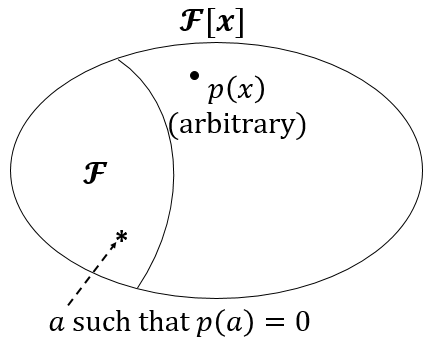
\includegraphics[scale=0.35]{images/algebraically_closed.png}
\caption{$F$ is algebraically closed: every $p(x)\in F[x]$ has an $a\in F$ such  $p(a)=0$.}\label{algebraicallyclosed}
\end{center}
\end{figure}

With this new definition in mind, we can restate Proposition~\ref{proposition:poly:FTOAhard} as follows: 

\begin{prop}{complexalgclosed}
$\mathbb{C}$ is algebraically closed.
\end{prop}

There are fields  besides $\mathbb{C}$ that are algebraically closed,  but there are  also  lots of fields that aren't:

\begin{exercise}{}
\begin {enumerate}[(a)]
\item
Are the rational numbers algebraically closed? Justify your answer.
\item
Are the real numbers algebraically closed? Justify your answer.
\end{enumerate}
\end{exercise}

%\begin{solution}{}
%\begin {enumerate}[(a)]
%\item
%Let $p(x)=x^2-2.$ $p(x)\in \mathbb{Q}[x]$, because $1, 2\in Q$. But the solutions $\pm \sqrt2\not\in Q$. Therefore, according to the defintion of algebraically closed, the field $Q$ is \textbf{not} algebraically closed.
%\item
%Let $p(x)=x^2+2.$ $p(x)\in \mathbb{R}[x]$, because $1, 2\in R$. But the solutions $\pm \sqrt2 i\not\in R$. Therefore, according to the defintion of algebraically closed, the field $R$ is \textbf{not} algebraically closed.
%\end{enumerate}
%\end{solution}

\begin{exercise}{}
\begin{enumerate}[(a)]
\item
In the field $\mathbb{Z}_5$, evaluate the polynomial $x^4+2$  for all elements of  $\mathbb{Z}_5$.
\item
Using part (a), show  that $\mathbb{Z}_5$ is not algebraically closed.
\item
Use the polynomial $x^6 + 2$ to determine whether or not $\mathbb{Z}_7$ is algebraically closed.
\end{enumerate}
\end{exercise}

\section{Field extensions and algebraic elements}
We've seen quite a few fields that are not algebraically closed. For example, the rational numbers $\mathbb{Q}$ are not algebraically closed, because e.g. $x^2 - 2$ has no  roots in $\mathbb{Q}$.  However, we were able to find a larger field (namely $\mathbb{R}$) that contains $\mathbb{Q}$ which has the root that $\mathbb{Q}$ is lacking. In this section, we'll talk about situations like this in a general context. 


First we need some general terminology to describe the case where one field is contained in  another:


\begin{defn}\label{def:subfield}  
Given a field $E$ and $F\subset E$, then $F$ is called a \term{subfield} of $E$ if $F$ is also a field with the same field operations as $E$. Conversely, $E$ is called an \term{extension field}\index{Field!extension} of $F$.
 \end{defn}

Now let's complete the following exercise to bolster our understanding of Definition~\ref{def:subfield}

\begin{exercise}{}
\begin{enumerate}[(a)]
\item
Give an example of a field $F$ that has a nontrivial extension field (that is, the extension field contains elements that are not in $F$).
\item
Give an example of a field, $F$ that is a subset of a field $E$, but is not a subfield of $E$. Explain.
\end{enumerate}
\end{exercise}

%\begin{solution}{}
%\begin{enumerate}[(a)]
%\item
%We know that $R\subset C$ and they have the same field operations. Therefore $R$ is a subfield of $C$ and $C$ is an extension field of $R$. The field extension is written as $C/R$.
%\item
%Consider the field, $Z_n\subset R$. The two fields do not have the same field operations, therefore $R/Z_n$ is not a field extension.
%\end{enumerate}
%\end{solution}

We also need terminology to describe roots of polynomials in $F[x]$ that aren't in $F$:

\begin{defn}\label{def:algover}  
Let $F$ be a subfield of $E$, and let $a\in E$. If $p(a)=0$ for some $p(x) \in F[x]$, then $a$ is \term*{algebraic}\index{Algebraic!element, of a field}\index{Field!algebraic element of} over $F$ (see Figure \ref{algebraicelement}). Otherwise, $a$  is \term*{transcendental}\index{Transcendental!element, of a field}\index{Field!transcendental element of} over $F$.
\end{defn}

\begin{figure}
\begin{center}
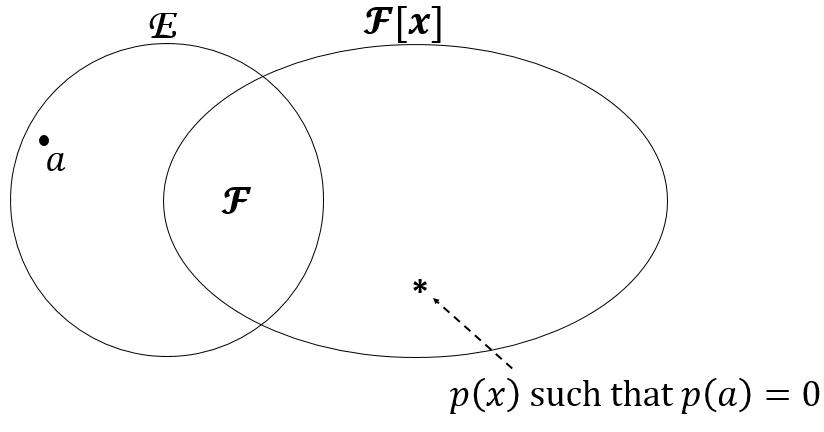
\includegraphics[scale=0.35]{images/algebraic_element.png}
\caption{$a\in E$ is algebraic over $F$:  there exists $p(x)\in F[x]$ such that $p(a)=0$.}\label{algebraicelement}
\end{center}
\end{figure}

\begin{exercise}{}
\begin {enumerate}[(a)]
\item
Give an example of an element of $\mathbb{C}\setminus \mathbb{R}$ which is algebraic over $\mathbb{Q}$. Justify your answer.
\item
Suppose that $z \in \mathbb{C}$ is algebraic over $\mathbb{R}$. Show that $\bar{z}$ is also algebraic over $\mathbb{R}$.
\item
Show that every element of $\mathbb{C}$ is algebraic over $\mathbb{R}$.
\end{enumerate}
\end{exercise}


\begin{exercise}{}
\begin {enumerate}[(a)]
\item
Given that $a \in \mathbb{C}$ is algebraic over $\mathbb{Q}$, show that $\sqrt{a}$ is also algebraic over $\mathbb{Q}$.
\item
Given that $a \in \mathbb{C}$ is algebraic over $\mathbb{Q}$, show that $a^{1/n}$ is also algebraic over $\mathbb{Q}$ for any natural number $n$.
\end{enumerate}
\end{exercise}


\begin{rem}\label{remark:poly:transcendental}
It's not so easy to show that elements are transcendental. This is because to show that $a$ is transcendental over $F$, you need to show that there's no polynomial whatsoever in $F[x]$  which has $a$ as a root. Let's consider in particular the case $F = \mathbb{Q}$. We saw in Chapter~\ref{complex} that $\mathbb{R}$ has lots of \emph{irrational} numbers, but so far we haven't definitely identified any real number that is transcendental over $\mathbb{Q}$. 

In 1844, Joseph Liouville gave the first proof that a transcendental number exists.  Liouville constructed a number (using infinite series) with special properties, and was able to show that it's impossible to construct a polynomial in $\mathbb{Q}[x]$ that has that number as a root. Hermite showed about 30 years later that $e$ was transcendental, and $\pi$ was added to the list (by Lindemann) 10 years after that. 

Even today, only  a handful of classes of numbers have been shown to be transcendental. This is not to say that there aren't lots of them. In fact, Georg Cantor in 1874 was able to show that ``almost all'' real numbers are transcendental over $\mathbb{Q}$. This is a fascinating topic, and there's lots of information on the Internet if you're interested in pursuing it further (one place to look is 
\url{http://mathworld.wolfram.com/TranscendentalNumber.html}).
\end{rem}

%\begin{solution}{}
%\begin {enumerate}[(a)]
%\item
%Consider $p(x)=x^2+3$. We see that $p(x)\in \mathbb{R}[x]$, because its coefficients are real. But the roots of $p(x)$ are $\pm \sqrt3 i$, which are not real. Also $R \subset C$ and they have the same field operations. Therefore, $\sqrt3 i$ and $-\sqrt{3}i$ are both algebraic over $R$.
%\item
%Consider the natural number $e\in R/Q$; which is not the root of any polynomial in $\mathbb{Q}[x]$. Also $Q\in R$ and they have the same field operations. Therefore, $e$ is transcendental over $R$.
%\item
%Consider $\pi\in C/Q$; which is not the root of any polynomial in $\mathbb{Q}[x]$. Also $Q\in R$ and they have the same field operations. Therefore, $\pi$ is transcendental over $Q$. Now let $p(x)=x-\pi\in \mathbb{R}[x]$. This shows that $\pi$ is the root of a polynomial in $\mathbb{R}[x]$ Therefore, $\pi$ is algebraic over $R$.
%\end{enumerate}
%\end{solution}

For field extensions which have no transcendental elements, the following definition applies:

\begin{defn}\label{def:algfieldextension}  
Suppose $E$ is an extension field of $F$. Then $E$ is called an \term{algebraic extension}\index{Field!algebraic extension} of $F$ if every $a\in E$ is algebraic over $F$. %Otherwise, $E$ is transcendental if it contains at least one $a$ such that $a$ is transcendental over $F$. 
%$E$ is called a \term{transcendental extension} of $F$.
 \end{defn}

\begin{exercise}{}
\begin{enumerate}[(a)]
\item
Give an example of a extension field that is algebraic. Justify your answer.
\item
Give an example of a field extension that is not algebraic. Justify your answer.
\end{enumerate}
\end{exercise}

A field extension may be algebraic, but still contain polynomials that have no roots. There's a special term for field extensions which contain roots for \emph{all} their polynomials:

%\begin{solution}{}
%\begin{enumerate}[(a)]
%\item
%Consider the field extension $C/R$. Every $a\in C$ can be shown to be a root of some polynomial in $\mathbb{R}[x]$. Therefore, every $a\in C$ is algebraic over $R$ and we say that $C/R$ is an algebraic field extension.
%\item
%Consider the field extension $R/Q$. We know that $\pi\in R$, but it can be shown that $\pi$ is not the root of any polynomail in $\mathbb{Q}[x]$. Therefore, $\pi$ is transcendental over $Q$ and we say that $R/Q$ is a transcendental field extension.
%\end{enumerate}
%\end{solution}

\begin{defn}\label{def:algclosure}  
Let $E$ be an algebraic extension field of $F$. Suppose that for every $p(x) \in E[x]$, there exists $a \in E$ such that $p(a)=0$.  Then  $E$ is  an \term*{algebraic closure}\index{Field!algebraic closure of}\index{Algebraic closure!of a field} of $F$ (see Figure \ref{algebraicclosure}).
\end{defn}

\begin{figure}
\begin{center}
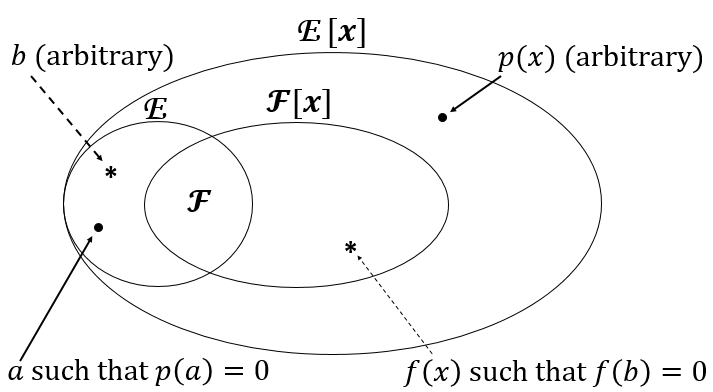
\includegraphics[scale=0.35]{images/algebraic_closure.png}
\caption{$E$ is an algebraic closure of $F$:  every $p(x)\in E[x]$ has an $a\in E$ such that $p(a)=0$; and every $b\in E$ has an $f(x)\in F[x]$ such that $f(b)=0$.}\label{algebraicclosure}
\end{center}
\end{figure}

Here's an example of an algebraic closure:

\begin{prop}{realalgclosure}
$\mathbb{C}$ is an algebraically closure of $\mathbb{R}$.
\end{prop}


\begin{proof}{}
Let $a+bi \in \mathbb{C}$ be arbitrary and let $p(x)=(x-(a+bi))(x-(a-bi))= x^2-2ax+a^2+b^2\in\mathbb{R}[x]$. We see that $a+bi$ is a root of $p(x)$. Since $a+bi$ is arbitrary, we can say that any element of $\mathbb{C}$ is a root of some polynomial in $\in\mathbb{R}[x]$. By Definition~\ref{def:algfieldextension} this makes $\mathbb{C}$ an algebraic extension of $\mathbb{R}$. Additionally, by Proposition~\ref{proposition:poly:complexalgclosed}, $\mathbb{C}$ is algebraically closed. Therefore, by Definition~\ref{def:algclosure}, $\mathbb{C}$ is the algebraic closure of $\mathbb{R}$.
\end{proof}

Does every field have an algebraic closure? Let's look at some field extensions we're already familiar with:

\begin{exercise}{}
\begin{enumerate}[(a)]
\item
Give an example that shows that $\mathbb{C}$ is not an algebraic closure of $\mathbb{Q}$ . Explain.
\item
Give an example that shows that $\mathbb{R}$ is not an algebraic closure of $\mathbb{Q}$ . Explain.
\end{enumerate}
\end{exercise}


Although we won't prove it here, it can be shown that every field has an algebraic closure:see  \url{https://soffer801.wordpress.com/2011/10/25/every-field-has-an-algebraic-closure/} for a nice discussion. In particular, there is a subfield of $\mathbb{C}$ which is an algebraic closure of $\mathbb{Q}$: this subfield is called the field of \term{algebraic numbers}.

\begin{exercise}{}
Draw a set diagram that shows the relationships between the sets $\mathbb{Q}, \mathbb{R}, \mathbb{C}$, and $\mathbb{A}$, where $\mathbb{A}$ denotes the set of algebraic numbers.  (For example, the ``set bubble'' representing $\mathbb{Q}$ should be inside the bubble representing $\mathbb{C}$, since $\mathbb{Q} \subset \mathbb{C}$.)
\end{exercise}

\section{Applications of algebraic field extensions}

We've already seen how field extensions play an important role in mathematics.  The irrational numbers were first introduced using an algebraic  field extension  of $\mathbb{Q}$  (although later it was discovered that not all irrational numbers are algebraic over $\mathbb{Q}$).  Similarly, the complex numbers were created as an algebraic field extension of the real numbers.  But this is just the beginning. Algebraic field extensions have played a pivotal role in a great number of deep mathematical results obtained over the last 200 years. Here is a short list of results which make use of algebraic field extensions:

\begin{itemize}
\item 
The quadratic formula expresses the roots of quadratic polynomials  in terms of algebraic operations on the coefficients plus a square root. There are similar (but vastly more complicated) formulas for solving cubic and quartic (3rd and 4th degree)  polynomial equations, which involve algebraic operations and  taking $n$th roots, for different values of $n$.  How about quintic (5th degree) polynomials?  Amazingly, it is possible to prove that there is no general formula for the solution of a quintic equation in terms of roots and algebraic operations.  Not just the formula is not known--there is \emph{no formula}. Period. This stupendous result is associated with the mathematicians Evariste Galois, Niels Henrik Abel, and Paolo Ruffini, and was proved in the mid-19th century.

This result relates to field extensions because every solution to an equation that involves only roots and algebraic operations must belong to certain type of field extension of the rationals. This fact imposes conditions on the type of numbers that can be expressed in such a form. It can be shown that there are roots of 5th-degree equations that don't meet these conditions---hence they can't possibly satisfy such an equation.

\item
Beginning with the Greeks,  mathematicians tried for thousands of years to find a way to trisect an angle, using only straightedge and compass. In 1837, Pierre Wantzel finally showed that it is \emph{impossible}: his proof built on previous results of Galois. (Think of how many hours over how many centuries were spent on a futile quest!)

This result relates to field extensions in similar fashion as the previous one. Geometrical points in the plane are identified as complex numbers (as we described in Section~\ref{complex_roots}). Every point constructed based on a set of  points is an algebraic combination of the corresponding complex numbers, together with square roots. This means that every constructable point must be contained in a series of field extensions created by successively adding square roots to an existing field. It can be shown that trisecting an angle involves finding a cube root which cannot possibly belong to such a series of extensions.  You may consult:

\noindent
 \url{https://terrytao.wordpress.com/2011/08/10/a-geometric-proof-of-the-impossibility-of-angle-trisection-by-straightedge-and-compass/}

\noindent
 to get a flavor of how this proof goes.
\item
A similar constructability problem is known as ``squaring the circle'':  Given a square of side 1, find a circle with the same area using only straightedge and compass. This can be shown to be impossible, as a consequence of the transcendence of $\pi$ alluded to in Remark~\ref{remark:poly:transcendental}.
\end{itemize}


% Applications of field extensions
% Field extensions and solvability of polynomial equations by radicals
% Give example of quadratic formula. There is a formula for cubic and quartic.  There is no formula for quintic. Not just the formula is not known--there is NO FORMULA. Proving this has to rank as one of the great intellectual achievements of all time.
% In this section, give you some idea of the methods involved in this proof.
% Show adding sqrt gives extension field.
% Consider quadratic formula. Shows that  the root is in extension field
% Add other square roots. produces another field extension.
% Transcendental over 


% Impossible constructions using straightedge and compass.
% Every complex number constructed based on a set of points  is the root of a quadratic equation 
% The set of all constructable points is contained in a field extension obtained by adding successive square roots.  This limits the types of numbers that can be constructed.
% Extension using square roots.  Can show that there are cube roots which are not in any field extension obtained in this manner.
%https://terrytao.wordpress.com/2011/08/10/a-geometric-proof-of-the-impossibility-of-angle-trisection-by-straightedge-and-compass/
% Squaring the circle. Amounts to constructing $\sqrt{\pi}$. If this is possible, then 
% Prove that if \sqrt{pi} is algebraic, then \pi is also algebraic.


%Now that we understand what it means for an element to be algebraic over or transcendental over a field, we can further our discussion into extension fields.  The theory of extension fields has played a critical role in the development of mathematics. For example, the ancient Greeks used geometry to construct rational numbers from line segments, but could not construct the square root of prime numbers, which they encountered  as hypotenuses of some right triangles.
% Irrational square roots give extension fields for the rational numbers
%$ a + b\sqrt{2}$ is an extension field of rationals
%real are extension field of rationals
%Before we go on with our discussion though, we must consider a couple of definitions.


%\begin{solution}
%Consider $\pi$. We know that $\pi\in C$, but it can be shown that $\pi$ is not the root of any polynomail in $\mathbb{Q}[x]$. Therefore, $C$ is not the algebraic closure of $Q$.
%\end{solution}

% Say something about extension fields
% The theory of extension fields has played a critical role in the development of mathematics. 
% Irrational square roots give extension fields for the rational numbers
% a + b\sqrt{2} is an extension field of rationals
%real are extension field of rationals
%e, pi, irrational that dont have
%if a set has no proper field extensions, then it is algebraically closed

%
%
%\section{Irreducible Polynomials}
% 
% 
%A nonconstant polynomial $f(x) \in F[x]$ is \term{
%irreducible}\index{Polynomial!irreducible}\index{Irreducible polynomial}
%over a field $F$ if $f(x)$ cannot be expressed as a product of two
%polynomials $g(x)$ and $h(x)$ in $F[x]$, where the degrees of $g(x)$
%and $h(x)$ are both smaller than the degree of $f(x)$.  Irreducible
%polynomials function as the ``prime numbers'' of polynomial rings.
% 
% 
%\begin{example}{poly_irred}
%The polynomial $x^2 - 2 \in {\mathbb Q}[x]$ is irreducible since it
%cannot be factored any further over the rational numbers. Similarly,
%$x^2 + 1$ is  irreducible over the real numbers. 
%\end{example}
% 
% 
%\begin{example}{finite_poly}
%The polynomial $p(x) = x^3 + x^2 + 2$ is irreducible over ${\mathbb
%Z}_3[x]$. Suppose that this polynomial was reducible over ${\mathbb
%Z}_3[x]$.  By the division algorithm there would have to be a factor
%of the form $x - a$, where $a$ is some element in ${\mathbb Z}_3[x]$.
%Hence, it would have to be true that $p(a) = 0$.  However,
%\begin{align*}
%p(0) & = 2 \\
%p(1) & = 1 \\
%p(2) & = 2.
%\end{align*}
%Therefore, $p(x)$ has no zeros in ${\mathbb Z}_3$ and must be
%irreducible. 
%\end{example}
%
%
%\begin{lemma}\label{poly:integer_coef_lemma}
%Let $p(x) \in {\mathbb Q}[x]$.  Then
%\[
%p(x) = \frac{r}{s}(a_0 + a_1 x + \cdots + a_n x^n),
%\]
%where $r, s, a_0, \ldots, a_n$ are integers, the $a_i$'s are
%relatively prime, and $r$ and $s$ are relatively prime. 
%\end{lemma}
% 
% 
%\begin{proof}
%Suppose that
%\[
%p(x) = \frac{b_0}{c_0} + \frac{b_1}{c_1} x + \cdots + \frac{b_n}{c_n}
%x^n,
%\]
%where the $b_i$'s and the $c_i$'s are integers. We can rewrite $p(x)$
%as 
%\[
%p(x) = \frac{1}{c_0 \cdots c_n} (d_0 + d_1 x + \cdots + d_n x^n),
%\]
%where $d_0, \ldots, d_n$ are integers. Let $d$ be the greatest common
%divisor of $d_0, \ldots, d_n$.  Then
%\[
%p(x) = \frac{d}{c_0 \cdots c_n} (a_0 + a_1 x + \cdots + a_n x^n),
%\]
%where $d_i = d a_i$ and the $a_i$'s are relatively prime. Reducing $d
%/(c_0 \cdots c_n)$ to its lowest terms, we can write
%\[
%p(x) = \frac{r}{s}(a_0 + a_1 x + \cdots + a_n x^n), 
%\]
%where $\gcd(r,s) = 1$.
%\end{proof}
